
% Default to the notebook output style

    


% Inherit from the specified cell style.




    
\documentclass[11pt]{article}

    
    
    \usepackage[T1]{fontenc}
    % Nicer default font (+ math font) than Computer Modern for most use cases
    \usepackage{mathpazo}

    % Basic figure setup, for now with no caption control since it's done
    % automatically by Pandoc (which extracts ![](path) syntax from Markdown).
    \usepackage{graphicx}
    % We will generate all images so they have a width \maxwidth. This means
    % that they will get their normal width if they fit onto the page, but
    % are scaled down if they would overflow the margins.
    \makeatletter
    \def\maxwidth{\ifdim\Gin@nat@width>\linewidth\linewidth
    \else\Gin@nat@width\fi}
    \makeatother
    \let\Oldincludegraphics\includegraphics
    % Set max figure width to be 80% of text width, for now hardcoded.
    \renewcommand{\includegraphics}[1]{\Oldincludegraphics[width=.8\maxwidth]{#1}}
    % Ensure that by default, figures have no caption (until we provide a
    % proper Figure object with a Caption API and a way to capture that
    % in the conversion process - todo).
    \usepackage{caption}
    \DeclareCaptionLabelFormat{nolabel}{}
    \captionsetup{labelformat=nolabel}

    \usepackage{adjustbox} % Used to constrain images to a maximum size 
    \usepackage{xcolor} % Allow colors to be defined
    \usepackage{enumerate} % Needed for markdown enumerations to work
    \usepackage{geometry} % Used to adjust the document margins
    \usepackage{amsmath} % Equations
    \usepackage{amssymb} % Equations
    \usepackage{textcomp} % defines textquotesingle
    % Hack from http://tex.stackexchange.com/a/47451/13684:
    \AtBeginDocument{%
        \def\PYZsq{\textquotesingle}% Upright quotes in Pygmentized code
    }
    \usepackage{upquote} % Upright quotes for verbatim code
    \usepackage{eurosym} % defines \euro
    \usepackage[mathletters]{ucs} % Extended unicode (utf-8) support
    \usepackage[utf8x]{inputenc} % Allow utf-8 characters in the tex document
    \usepackage{fancyvrb} % verbatim replacement that allows latex
    \usepackage{grffile} % extends the file name processing of package graphics 
                         % to support a larger range 
    % The hyperref package gives us a pdf with properly built
    % internal navigation ('pdf bookmarks' for the table of contents,
    % internal cross-reference links, web links for URLs, etc.)
    \usepackage{hyperref}
    \usepackage{longtable} % longtable support required by pandoc >1.10
    \usepackage{booktabs}  % table support for pandoc > 1.12.2
    \usepackage[inline]{enumitem} % IRkernel/repr support (it uses the enumerate* environment)
    \usepackage[normalem]{ulem} % ulem is needed to support strikethroughs (\sout)
                                % normalem makes italics be italics, not underlines
    

    
    
    % Colors for the hyperref package
    \definecolor{urlcolor}{rgb}{0,.145,.698}
    \definecolor{linkcolor}{rgb}{.71,0.21,0.01}
    \definecolor{citecolor}{rgb}{.12,.54,.11}

    % ANSI colors
    \definecolor{ansi-black}{HTML}{3E424D}
    \definecolor{ansi-black-intense}{HTML}{282C36}
    \definecolor{ansi-red}{HTML}{E75C58}
    \definecolor{ansi-red-intense}{HTML}{B22B31}
    \definecolor{ansi-green}{HTML}{00A250}
    \definecolor{ansi-green-intense}{HTML}{007427}
    \definecolor{ansi-yellow}{HTML}{DDB62B}
    \definecolor{ansi-yellow-intense}{HTML}{B27D12}
    \definecolor{ansi-blue}{HTML}{208FFB}
    \definecolor{ansi-blue-intense}{HTML}{0065CA}
    \definecolor{ansi-magenta}{HTML}{D160C4}
    \definecolor{ansi-magenta-intense}{HTML}{A03196}
    \definecolor{ansi-cyan}{HTML}{60C6C8}
    \definecolor{ansi-cyan-intense}{HTML}{258F8F}
    \definecolor{ansi-white}{HTML}{C5C1B4}
    \definecolor{ansi-white-intense}{HTML}{A1A6B2}

    % commands and environments needed by pandoc snippets
    % extracted from the output of `pandoc -s`
    \providecommand{\tightlist}{%
      \setlength{\itemsep}{0pt}\setlength{\parskip}{0pt}}
    \DefineVerbatimEnvironment{Highlighting}{Verbatim}{commandchars=\\\{\}}
    % Add ',fontsize=\small' for more characters per line
    \newenvironment{Shaded}{}{}
    \newcommand{\KeywordTok}[1]{\textcolor[rgb]{0.00,0.44,0.13}{\textbf{{#1}}}}
    \newcommand{\DataTypeTok}[1]{\textcolor[rgb]{0.56,0.13,0.00}{{#1}}}
    \newcommand{\DecValTok}[1]{\textcolor[rgb]{0.25,0.63,0.44}{{#1}}}
    \newcommand{\BaseNTok}[1]{\textcolor[rgb]{0.25,0.63,0.44}{{#1}}}
    \newcommand{\FloatTok}[1]{\textcolor[rgb]{0.25,0.63,0.44}{{#1}}}
    \newcommand{\CharTok}[1]{\textcolor[rgb]{0.25,0.44,0.63}{{#1}}}
    \newcommand{\StringTok}[1]{\textcolor[rgb]{0.25,0.44,0.63}{{#1}}}
    \newcommand{\CommentTok}[1]{\textcolor[rgb]{0.38,0.63,0.69}{\textit{{#1}}}}
    \newcommand{\OtherTok}[1]{\textcolor[rgb]{0.00,0.44,0.13}{{#1}}}
    \newcommand{\AlertTok}[1]{\textcolor[rgb]{1.00,0.00,0.00}{\textbf{{#1}}}}
    \newcommand{\FunctionTok}[1]{\textcolor[rgb]{0.02,0.16,0.49}{{#1}}}
    \newcommand{\RegionMarkerTok}[1]{{#1}}
    \newcommand{\ErrorTok}[1]{\textcolor[rgb]{1.00,0.00,0.00}{\textbf{{#1}}}}
    \newcommand{\NormalTok}[1]{{#1}}
    
    % Additional commands for more recent versions of Pandoc
    \newcommand{\ConstantTok}[1]{\textcolor[rgb]{0.53,0.00,0.00}{{#1}}}
    \newcommand{\SpecialCharTok}[1]{\textcolor[rgb]{0.25,0.44,0.63}{{#1}}}
    \newcommand{\VerbatimStringTok}[1]{\textcolor[rgb]{0.25,0.44,0.63}{{#1}}}
    \newcommand{\SpecialStringTok}[1]{\textcolor[rgb]{0.73,0.40,0.53}{{#1}}}
    \newcommand{\ImportTok}[1]{{#1}}
    \newcommand{\DocumentationTok}[1]{\textcolor[rgb]{0.73,0.13,0.13}{\textit{{#1}}}}
    \newcommand{\AnnotationTok}[1]{\textcolor[rgb]{0.38,0.63,0.69}{\textbf{\textit{{#1}}}}}
    \newcommand{\CommentVarTok}[1]{\textcolor[rgb]{0.38,0.63,0.69}{\textbf{\textit{{#1}}}}}
    \newcommand{\VariableTok}[1]{\textcolor[rgb]{0.10,0.09,0.49}{{#1}}}
    \newcommand{\ControlFlowTok}[1]{\textcolor[rgb]{0.00,0.44,0.13}{\textbf{{#1}}}}
    \newcommand{\OperatorTok}[1]{\textcolor[rgb]{0.40,0.40,0.40}{{#1}}}
    \newcommand{\BuiltInTok}[1]{{#1}}
    \newcommand{\ExtensionTok}[1]{{#1}}
    \newcommand{\PreprocessorTok}[1]{\textcolor[rgb]{0.74,0.48,0.00}{{#1}}}
    \newcommand{\AttributeTok}[1]{\textcolor[rgb]{0.49,0.56,0.16}{{#1}}}
    \newcommand{\InformationTok}[1]{\textcolor[rgb]{0.38,0.63,0.69}{\textbf{\textit{{#1}}}}}
    \newcommand{\WarningTok}[1]{\textcolor[rgb]{0.38,0.63,0.69}{\textbf{\textit{{#1}}}}}
    
    
    % Define a nice break command that doesn't care if a line doesn't already
    % exist.
    \def\br{\hspace*{\fill} \\* }
    % Math Jax compatability definitions
    \def\gt{>}
    \def\lt{<}
    % Document parameters
    \title{Shor's Algorithm}
    
    
    

    % Pygments definitions
    
\makeatletter
\def\PY@reset{\let\PY@it=\relax \let\PY@bf=\relax%
    \let\PY@ul=\relax \let\PY@tc=\relax%
    \let\PY@bc=\relax \let\PY@ff=\relax}
\def\PY@tok#1{\csname PY@tok@#1\endcsname}
\def\PY@toks#1+{\ifx\relax#1\empty\else%
    \PY@tok{#1}\expandafter\PY@toks\fi}
\def\PY@do#1{\PY@bc{\PY@tc{\PY@ul{%
    \PY@it{\PY@bf{\PY@ff{#1}}}}}}}
\def\PY#1#2{\PY@reset\PY@toks#1+\relax+\PY@do{#2}}

\expandafter\def\csname PY@tok@w\endcsname{\def\PY@tc##1{\textcolor[rgb]{0.73,0.73,0.73}{##1}}}
\expandafter\def\csname PY@tok@c\endcsname{\let\PY@it=\textit\def\PY@tc##1{\textcolor[rgb]{0.25,0.50,0.50}{##1}}}
\expandafter\def\csname PY@tok@cp\endcsname{\def\PY@tc##1{\textcolor[rgb]{0.74,0.48,0.00}{##1}}}
\expandafter\def\csname PY@tok@k\endcsname{\let\PY@bf=\textbf\def\PY@tc##1{\textcolor[rgb]{0.00,0.50,0.00}{##1}}}
\expandafter\def\csname PY@tok@kp\endcsname{\def\PY@tc##1{\textcolor[rgb]{0.00,0.50,0.00}{##1}}}
\expandafter\def\csname PY@tok@kt\endcsname{\def\PY@tc##1{\textcolor[rgb]{0.69,0.00,0.25}{##1}}}
\expandafter\def\csname PY@tok@o\endcsname{\def\PY@tc##1{\textcolor[rgb]{0.40,0.40,0.40}{##1}}}
\expandafter\def\csname PY@tok@ow\endcsname{\let\PY@bf=\textbf\def\PY@tc##1{\textcolor[rgb]{0.67,0.13,1.00}{##1}}}
\expandafter\def\csname PY@tok@nb\endcsname{\def\PY@tc##1{\textcolor[rgb]{0.00,0.50,0.00}{##1}}}
\expandafter\def\csname PY@tok@nf\endcsname{\def\PY@tc##1{\textcolor[rgb]{0.00,0.00,1.00}{##1}}}
\expandafter\def\csname PY@tok@nc\endcsname{\let\PY@bf=\textbf\def\PY@tc##1{\textcolor[rgb]{0.00,0.00,1.00}{##1}}}
\expandafter\def\csname PY@tok@nn\endcsname{\let\PY@bf=\textbf\def\PY@tc##1{\textcolor[rgb]{0.00,0.00,1.00}{##1}}}
\expandafter\def\csname PY@tok@ne\endcsname{\let\PY@bf=\textbf\def\PY@tc##1{\textcolor[rgb]{0.82,0.25,0.23}{##1}}}
\expandafter\def\csname PY@tok@nv\endcsname{\def\PY@tc##1{\textcolor[rgb]{0.10,0.09,0.49}{##1}}}
\expandafter\def\csname PY@tok@no\endcsname{\def\PY@tc##1{\textcolor[rgb]{0.53,0.00,0.00}{##1}}}
\expandafter\def\csname PY@tok@nl\endcsname{\def\PY@tc##1{\textcolor[rgb]{0.63,0.63,0.00}{##1}}}
\expandafter\def\csname PY@tok@ni\endcsname{\let\PY@bf=\textbf\def\PY@tc##1{\textcolor[rgb]{0.60,0.60,0.60}{##1}}}
\expandafter\def\csname PY@tok@na\endcsname{\def\PY@tc##1{\textcolor[rgb]{0.49,0.56,0.16}{##1}}}
\expandafter\def\csname PY@tok@nt\endcsname{\let\PY@bf=\textbf\def\PY@tc##1{\textcolor[rgb]{0.00,0.50,0.00}{##1}}}
\expandafter\def\csname PY@tok@nd\endcsname{\def\PY@tc##1{\textcolor[rgb]{0.67,0.13,1.00}{##1}}}
\expandafter\def\csname PY@tok@s\endcsname{\def\PY@tc##1{\textcolor[rgb]{0.73,0.13,0.13}{##1}}}
\expandafter\def\csname PY@tok@sd\endcsname{\let\PY@it=\textit\def\PY@tc##1{\textcolor[rgb]{0.73,0.13,0.13}{##1}}}
\expandafter\def\csname PY@tok@si\endcsname{\let\PY@bf=\textbf\def\PY@tc##1{\textcolor[rgb]{0.73,0.40,0.53}{##1}}}
\expandafter\def\csname PY@tok@se\endcsname{\let\PY@bf=\textbf\def\PY@tc##1{\textcolor[rgb]{0.73,0.40,0.13}{##1}}}
\expandafter\def\csname PY@tok@sr\endcsname{\def\PY@tc##1{\textcolor[rgb]{0.73,0.40,0.53}{##1}}}
\expandafter\def\csname PY@tok@ss\endcsname{\def\PY@tc##1{\textcolor[rgb]{0.10,0.09,0.49}{##1}}}
\expandafter\def\csname PY@tok@sx\endcsname{\def\PY@tc##1{\textcolor[rgb]{0.00,0.50,0.00}{##1}}}
\expandafter\def\csname PY@tok@m\endcsname{\def\PY@tc##1{\textcolor[rgb]{0.40,0.40,0.40}{##1}}}
\expandafter\def\csname PY@tok@gh\endcsname{\let\PY@bf=\textbf\def\PY@tc##1{\textcolor[rgb]{0.00,0.00,0.50}{##1}}}
\expandafter\def\csname PY@tok@gu\endcsname{\let\PY@bf=\textbf\def\PY@tc##1{\textcolor[rgb]{0.50,0.00,0.50}{##1}}}
\expandafter\def\csname PY@tok@gd\endcsname{\def\PY@tc##1{\textcolor[rgb]{0.63,0.00,0.00}{##1}}}
\expandafter\def\csname PY@tok@gi\endcsname{\def\PY@tc##1{\textcolor[rgb]{0.00,0.63,0.00}{##1}}}
\expandafter\def\csname PY@tok@gr\endcsname{\def\PY@tc##1{\textcolor[rgb]{1.00,0.00,0.00}{##1}}}
\expandafter\def\csname PY@tok@ge\endcsname{\let\PY@it=\textit}
\expandafter\def\csname PY@tok@gs\endcsname{\let\PY@bf=\textbf}
\expandafter\def\csname PY@tok@gp\endcsname{\let\PY@bf=\textbf\def\PY@tc##1{\textcolor[rgb]{0.00,0.00,0.50}{##1}}}
\expandafter\def\csname PY@tok@go\endcsname{\def\PY@tc##1{\textcolor[rgb]{0.53,0.53,0.53}{##1}}}
\expandafter\def\csname PY@tok@gt\endcsname{\def\PY@tc##1{\textcolor[rgb]{0.00,0.27,0.87}{##1}}}
\expandafter\def\csname PY@tok@err\endcsname{\def\PY@bc##1{\setlength{\fboxsep}{0pt}\fcolorbox[rgb]{1.00,0.00,0.00}{1,1,1}{\strut ##1}}}
\expandafter\def\csname PY@tok@kc\endcsname{\let\PY@bf=\textbf\def\PY@tc##1{\textcolor[rgb]{0.00,0.50,0.00}{##1}}}
\expandafter\def\csname PY@tok@kd\endcsname{\let\PY@bf=\textbf\def\PY@tc##1{\textcolor[rgb]{0.00,0.50,0.00}{##1}}}
\expandafter\def\csname PY@tok@kn\endcsname{\let\PY@bf=\textbf\def\PY@tc##1{\textcolor[rgb]{0.00,0.50,0.00}{##1}}}
\expandafter\def\csname PY@tok@kr\endcsname{\let\PY@bf=\textbf\def\PY@tc##1{\textcolor[rgb]{0.00,0.50,0.00}{##1}}}
\expandafter\def\csname PY@tok@bp\endcsname{\def\PY@tc##1{\textcolor[rgb]{0.00,0.50,0.00}{##1}}}
\expandafter\def\csname PY@tok@fm\endcsname{\def\PY@tc##1{\textcolor[rgb]{0.00,0.00,1.00}{##1}}}
\expandafter\def\csname PY@tok@vc\endcsname{\def\PY@tc##1{\textcolor[rgb]{0.10,0.09,0.49}{##1}}}
\expandafter\def\csname PY@tok@vg\endcsname{\def\PY@tc##1{\textcolor[rgb]{0.10,0.09,0.49}{##1}}}
\expandafter\def\csname PY@tok@vi\endcsname{\def\PY@tc##1{\textcolor[rgb]{0.10,0.09,0.49}{##1}}}
\expandafter\def\csname PY@tok@vm\endcsname{\def\PY@tc##1{\textcolor[rgb]{0.10,0.09,0.49}{##1}}}
\expandafter\def\csname PY@tok@sa\endcsname{\def\PY@tc##1{\textcolor[rgb]{0.73,0.13,0.13}{##1}}}
\expandafter\def\csname PY@tok@sb\endcsname{\def\PY@tc##1{\textcolor[rgb]{0.73,0.13,0.13}{##1}}}
\expandafter\def\csname PY@tok@sc\endcsname{\def\PY@tc##1{\textcolor[rgb]{0.73,0.13,0.13}{##1}}}
\expandafter\def\csname PY@tok@dl\endcsname{\def\PY@tc##1{\textcolor[rgb]{0.73,0.13,0.13}{##1}}}
\expandafter\def\csname PY@tok@s2\endcsname{\def\PY@tc##1{\textcolor[rgb]{0.73,0.13,0.13}{##1}}}
\expandafter\def\csname PY@tok@sh\endcsname{\def\PY@tc##1{\textcolor[rgb]{0.73,0.13,0.13}{##1}}}
\expandafter\def\csname PY@tok@s1\endcsname{\def\PY@tc##1{\textcolor[rgb]{0.73,0.13,0.13}{##1}}}
\expandafter\def\csname PY@tok@mb\endcsname{\def\PY@tc##1{\textcolor[rgb]{0.40,0.40,0.40}{##1}}}
\expandafter\def\csname PY@tok@mf\endcsname{\def\PY@tc##1{\textcolor[rgb]{0.40,0.40,0.40}{##1}}}
\expandafter\def\csname PY@tok@mh\endcsname{\def\PY@tc##1{\textcolor[rgb]{0.40,0.40,0.40}{##1}}}
\expandafter\def\csname PY@tok@mi\endcsname{\def\PY@tc##1{\textcolor[rgb]{0.40,0.40,0.40}{##1}}}
\expandafter\def\csname PY@tok@il\endcsname{\def\PY@tc##1{\textcolor[rgb]{0.40,0.40,0.40}{##1}}}
\expandafter\def\csname PY@tok@mo\endcsname{\def\PY@tc##1{\textcolor[rgb]{0.40,0.40,0.40}{##1}}}
\expandafter\def\csname PY@tok@ch\endcsname{\let\PY@it=\textit\def\PY@tc##1{\textcolor[rgb]{0.25,0.50,0.50}{##1}}}
\expandafter\def\csname PY@tok@cm\endcsname{\let\PY@it=\textit\def\PY@tc##1{\textcolor[rgb]{0.25,0.50,0.50}{##1}}}
\expandafter\def\csname PY@tok@cpf\endcsname{\let\PY@it=\textit\def\PY@tc##1{\textcolor[rgb]{0.25,0.50,0.50}{##1}}}
\expandafter\def\csname PY@tok@c1\endcsname{\let\PY@it=\textit\def\PY@tc##1{\textcolor[rgb]{0.25,0.50,0.50}{##1}}}
\expandafter\def\csname PY@tok@cs\endcsname{\let\PY@it=\textit\def\PY@tc##1{\textcolor[rgb]{0.25,0.50,0.50}{##1}}}

\def\PYZbs{\char`\\}
\def\PYZus{\char`\_}
\def\PYZob{\char`\{}
\def\PYZcb{\char`\}}
\def\PYZca{\char`\^}
\def\PYZam{\char`\&}
\def\PYZlt{\char`\<}
\def\PYZgt{\char`\>}
\def\PYZsh{\char`\#}
\def\PYZpc{\char`\%}
\def\PYZdl{\char`\$}
\def\PYZhy{\char`\-}
\def\PYZsq{\char`\'}
\def\PYZdq{\char`\"}
\def\PYZti{\char`\~}
% for compatibility with earlier versions
\def\PYZat{@}
\def\PYZlb{[}
\def\PYZrb{]}
\makeatother


    % Exact colors from NB
    \definecolor{incolor}{rgb}{0.0, 0.0, 0.5}
    \definecolor{outcolor}{rgb}{0.545, 0.0, 0.0}



    
    % Prevent overflowing lines due to hard-to-break entities
    \sloppy 
    % Setup hyperref package
    \hypersetup{
      breaklinks=true,  % so long urls are correctly broken across lines
      colorlinks=true,
      urlcolor=urlcolor,
      linkcolor=linkcolor,
      citecolor=citecolor,
      }
    % Slightly bigger margins than the latex defaults
    
    \geometry{verbose,tmargin=1in,bmargin=1in,lmargin=1in,rmargin=1in}
    
    

    \begin{document}
    
    
    \maketitle
    
    

    
    \hypertarget{shors-algorithm}{%
\section{Shor's Algorithm}\label{shors-algorithm}}

\emph{Mat Jones} \emph{CS360}

    \hypertarget{abstract}{%
\subsection{Abstract}\label{abstract}}

~~~~Although all integers have a unique breakdown of prime factors,
finding those prime factors is thought to be a hard problem in computer
science; in fact, most modern cyber security and encryption measures
depend on the assumption that solving this problem for integers of a
thousand or more digits is not feasibly possible (``Shor's Algorithm'').
However, in 1995, MIT professor Peter Shor presented a quantum algorithm
(an algorithm that runs on a quantum computer) to solve the factoring
problem in polynomial time. Shor's algorithm thus drastically changed
the set of problems in computer science that can be considered feasible.

    \hypertarget{introduction}{%
\subsection{Introduction}\label{introduction}}

~~~~Shor's algorithm could potentially break nearly all modern
cryptography. Most encryption schemes use a public \& private key
paradigm; each device has two keys (public and private key), and the
public keys are exchanged between devices. The keys are generated such
that data encrypted using the public key can only be decrypted using the
private key. Since the keys must be mathematically related (often based
on arithmetic involving prime factors), the private key can
theoretically be calculated from the public key. However, finding the
prime factors of an integer of a thousand digits or more becomes
infeasible on a classical computer; thus, calculating the private key
from the public key could take hundreds of years on a classical
computer, depending on the encryption scheme used.

Shor's algorithm is a quantum algorithm for efficiently finding the
prime factors of large integers, and thus calculating a private key from
a public key could become a feasible problem in the near future. For
this reason, it is important that software professionals prepare for the
eventuality of accessible quantum computing. While theoretically
effective post-quantum cryptography has been proposed, existing cyber
security infrastructure (made up of classical computers) is not equipped
to protect against attacks by a quantum computer.

    \hypertarget{implementation}{%
\subsection{Implementation}\label{implementation}}

\hypertarget{period-finding}{%
\subsubsection{Period Finding}\label{period-finding}}

~~~~It has been widely known by mathematicians and computer scientists
since the 1970's that the factorization problem becomes easy if given a
``period finding machine''; that is, a machine which can efficiently
find a period of the modular exponentiation function (``Shor's
Algorithm'').

The period finding problem is defined as follows: Given two integers
\(N\) and \(a\), find the smallest possible integer \(r\) such that
\(a^r-1\) is a multiple of \(N\). The number \(r\) is the period of
\(a\mod N\). Or, more simply, find the minimum possible value for \(r\)
such that:

\[a^{x+r} = a^x\pmod N\]

where \(x\) is any integer. Consider the following example for \(N=15\)
and \(a=7\):

\[7^2=4\pmod{15}=4\] \[7^3=4\times 7=13\pmod{15}=13\]
\[7^4=13\times 7=91\pmod{15}=1\]

This sequence gives rise to the pattern \(7^{x+4}=7^x\pmod{15}\), and
thus \(r=4\) is the period of the modular exponentiation function
\(7\pmod{15}\).

    \hypertarget{using-period-finding-machine-to-find-prime-factors}{%
\subsubsection{Using Period Finding Machine to Find Prime
Factors}\label{using-period-finding-machine-to-find-prime-factors}}

~~~~Suppose a period finding machine is given that takes two co-prime
integers \(a\) and \(N\) and outputs the period of \(a\mod N\). Then,
the prime factors \(p_1, p_2\) of \(N\) can be found by the following
procedure: 1. Choose a random integer \(a\) between \(2..N-1\). 2.
Compute the greatest common divisor (GCD) of \(a\) and \(N\) (can be
calculated efficiently using
\href{https://en.wikipedia.org/wiki/Euclidean_algorithm}{Euclid's
algorithm}); if this value is not equal to \(1\), then it equals either
\(p_1\) or \(p_2\), and the other can be computed from the found factor
(e.g. \(N/p_1\) or \(N/p_2\)). Otherwise, continue. 3. Let \(r\) be the
period of \(a\mod N\); repeat steps 1-3 until \(r\) is even. At this
point, a value for \(r\) has been found such that \(a^r-1\) is a
multiple of \(N\). 4. Consider the following identity:
\[a^r-1=(a^{r/2}-1)(a^{r/2}+1)\]

Thus, \(a^{r/2}-1\) is not a multiple of \(N\) (or else \(r\) would
equal \(r/2\)). If \(a^{r/2}+1\) is a multiple of \(N\), return to step
1. Otherwise, this means that neither of the values \(a^{r/2}\pm 1\) are
multiples of \(N\), but the product of these two values \emph{is} a
multiple of \(N\). This is possible if and only if \(p_1\) is a prime
factor of \(a^{r/2}-1\) and \(p_2\) is a prime factor of \(a^{r/2}+1\)
or vice versa. Therefore, \(p_1\) and \(p_2\) can now be computed by
\(p_1=GCD(N, a^{r/2}-1)\) and \(p_2=GCD(N, a^{r/2}+1)\). Consider the
following table showing the calculated prime factors of \(N=15\) given
different \(a\) values:

\begin{figure}
\centering
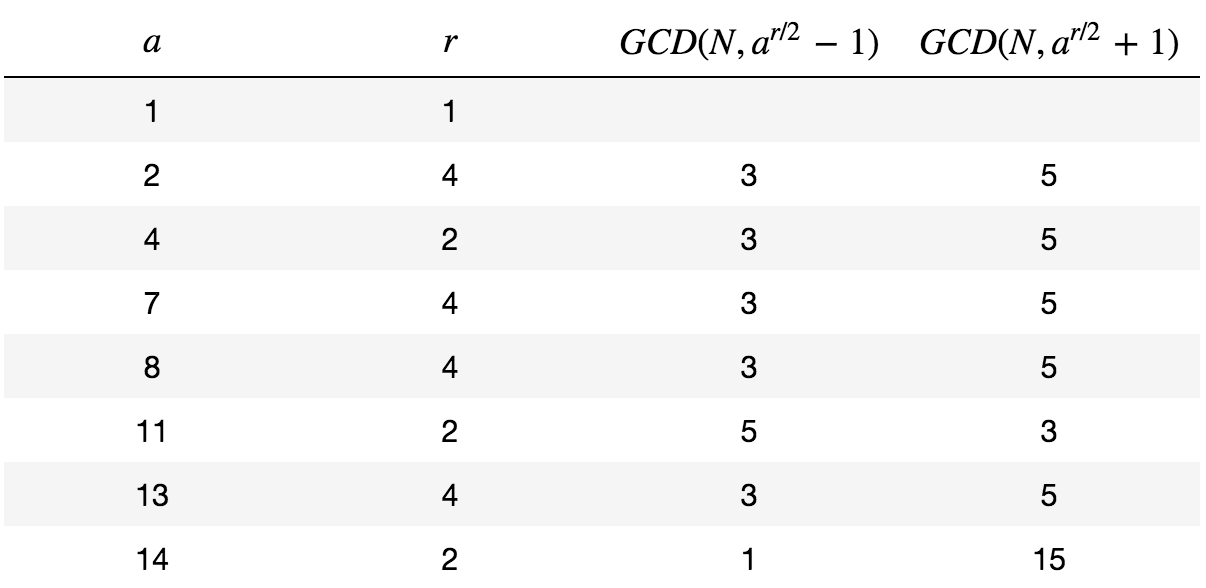
\includegraphics{table.png}
\caption{Table}
\end{figure}

Notice that \(a=14\) is the only ``unlucky'' integer chosen (i.e.~it
results in \(GCD(N, a^{r/2}+1)\) being a multiple of \(N\)); in general,
it can be shown that selection of ``unlucky'' integers are rather
infrequent (``Shor's Algorithm'').

    \hypertarget{using-a-quantum-computer-to-simulate-period-finding-machine}{%
\subsubsection{Using a Quantum Computer to Simulate Period Finding
Machine}\label{using-a-quantum-computer-to-simulate-period-finding-machine}}

~~~~The true power of Shor's algorithm lies in the ability of a quantum
computer to simulate such a ``period finding machine'' required to
efficiently solve the factoring problem. By exploiting quantum
parallelism and constructive interference, certain ``global properties''
can be derived from a complex function. The Deutsch-Jozsa algorithm uses
this technique to determine if a function has the global property of
being a balanced function (``Deutsch-Jozsa Algorithm''). In Shor's
algorithm, it can be used to determine the periodicity of the modular
exponentiation function.

Suppose two co-prime integers \(a\) and \(N\) are given; the goal is to
find the smallest possible integer \(r\) such that \(a^r=1\pmod N\). A
unitary operator \(U_a\) can be constructed which implements the modular
multiplication function such that \(U_a: x\rightarrow ax\pmod N\). With
this definition of \(U_a\), it can be shown that the each Eigenvalue of
\(U_a\) is of the form \(e^{i\phi}\) where \(\phi=2\pi k/r\) for some
integer \(k\) (``Shor's Algorithm'').

Eigenvalues of a unitary operator can be efficiently measured using the
quantum phase estimation algorithm (``Quantum Phase Estimation'').
However, the value of \(r\) can only be derived from a given Eigenvalue
if the Eigenvalue is measured \emph{exactly} or with exponentially small
precision; for example, a factorization of a \(1000\) digit integer
would require an Eigenvalue measured with a precision of \(10^{-2000}\)
(``Shor's Algorithm''). Such a level of precision cannot be achieved
using the phase estimation algorithm because it would require too large
a pointer system.

Instead, define a family of unitary operators \(U_b\) with
\(b=a, a^2, a^4, a^8,\dots a^{2^P}\) where \(P\approx N^2\). Notice that
all \(U_b\) are integer powers of \(U_a\); thus, if \(b=a^t\) for some
integer \(t\), then \(U_b=(U_a)^t\), which implies that all \(U_b\) have
the same Eigenvectors as \(U_a\). Further, this means that the
Eigenvalues of all \(U_b\) can be derived simultaneously. Additionally,
the implementation of \(U_b\) is as easy as implementing \(U_a\); simply
pre-compute the powers of \(U_a\) by repeated squaring method.
Conveniently, each squaring of \(a\) reduces the margin of error in the
estimation of \(U_a\) by a factor of \(1/_2\); this mitigates the
requirement for exact or exponentially small precision in the phase
estimation algorithm. For example, a precision of \(10^{-2000}\) can be
achieved by a series of \(10^6\) less precise measurements (up to 10\%
error) of \(U_b\), and selecting a few Eigenvalues \(\phi=2\pi k/r\) at
random to estimate with a precision of \(1/N^2\) is enough to derive an
exact value of \(r\) using rational approximation to estimate \(k/r\)
(``Shor's Algorithm'').

    \hypertarget{reversible-classical-circuits}{%
\paragraph{Reversible Classical
Circuits}\label{reversible-classical-circuits}}

~~~~A quantum circuit which implements the modular multiplication
operator is required in order to use the phase estimation gate. Quantum
algorithms can call classical subroutines if the classical subroutine is
first transformed into a \emph{reversible form}, i.e.~represented by a
sequence of reversible logic gates (CNOT gate, Toffoli gate, etc). That
is, the number of input wires must equal the number of output wires for
each gate. Further, the classical subroutine can use scratch memory for
local variables, but the scratch memory must be wiped clean upon
termination of the subroutine; leaving residual values in the scratch
memory could potentially destroy quantum coherence, preventing the
quantum routine from being able to detect interference between quantum
states (``Shor's Algorithm'').

Consider a standard AND gate; it can be transformed into a reversible
equivalent (R-AND) by adding an extra input wire \(d\) (so, inputs
\(a, b, d\)), which is a dummy wire expecting a value of \(d=0\), and
adding two extra output wires (so, outputs \(a, b, c\)) where \(c\) is
the result of \(d\oplus (a\wedge b)\) (see figure 1). Thus, all inputs
of the R-AND can be derived from its outputs since
\(c=d\oplus (a\wedge b)\) (``Shor's Algorithm'').

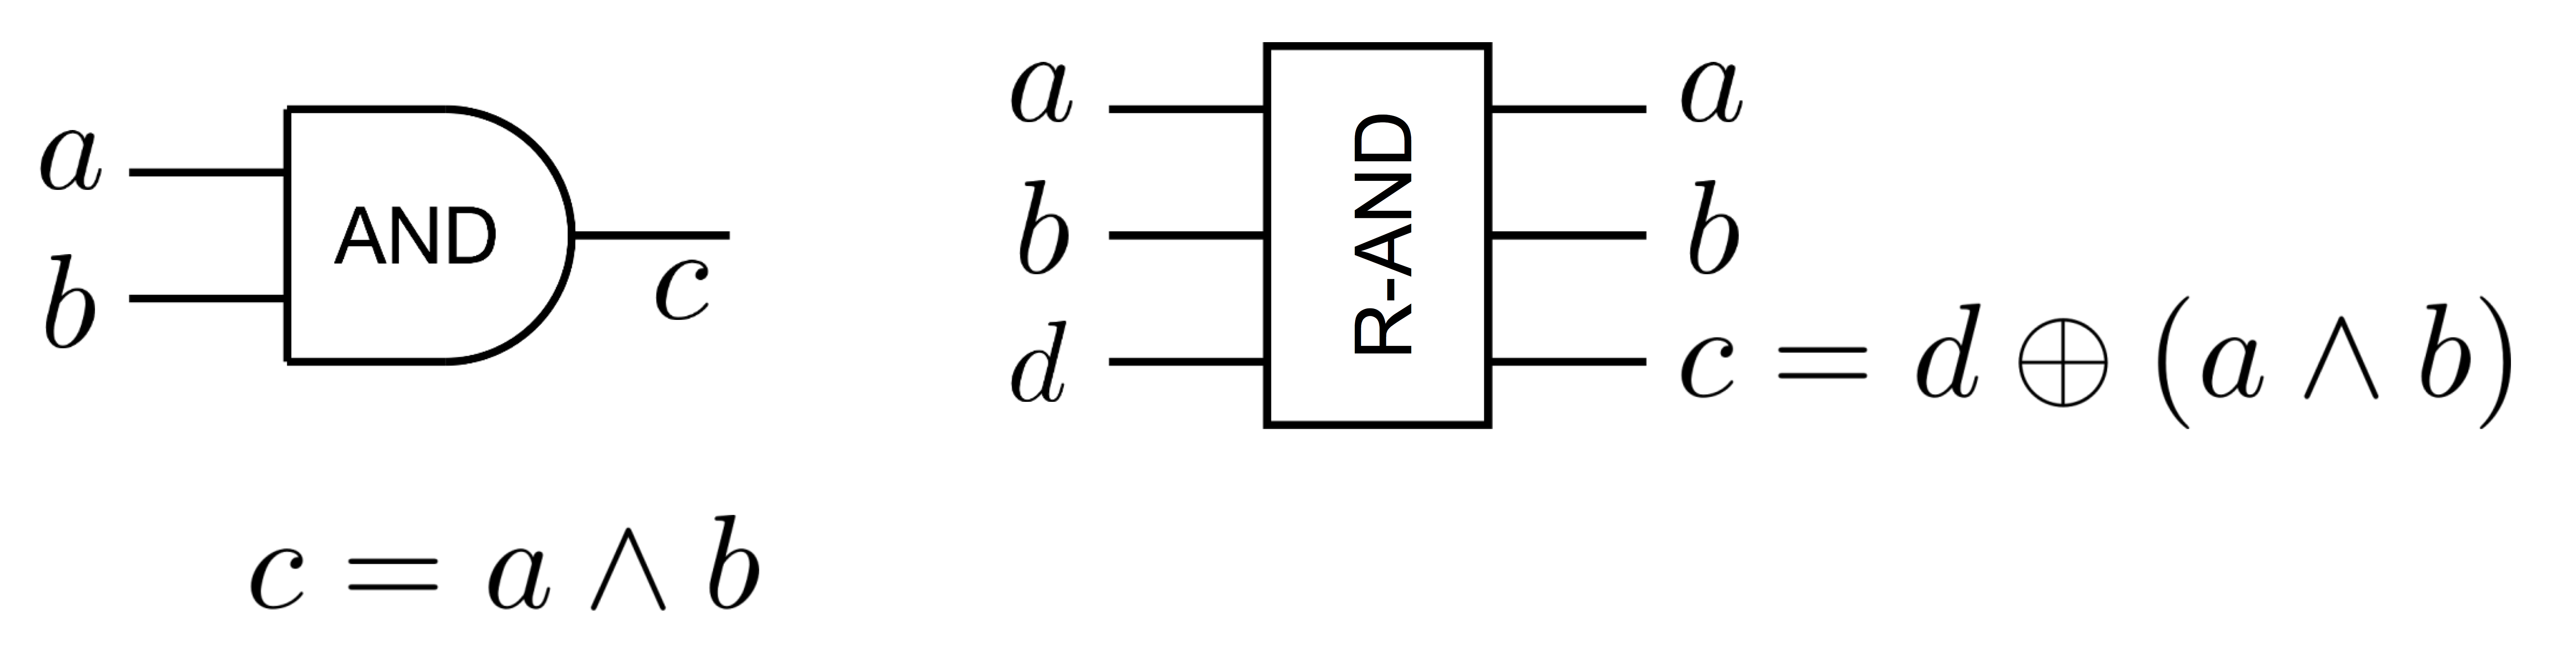
\includegraphics{r-and-gate.png}

\emph{Figure 1: Reversible AND (R-AND) gate. (Source: ``Shor's
Algorithm''})

 Similar logic can be applied to any gate with two inputs and one
output; if gate F computes a boolean function \(c=F(a,b)\), then a
reversible transformation (R-F gate) would map inputs \(a, b, d\) to
outputs \(a, b, c\) where \(c=d\oplus F(a, b)\) (``Shor's Algorithm'').
See figure 2.

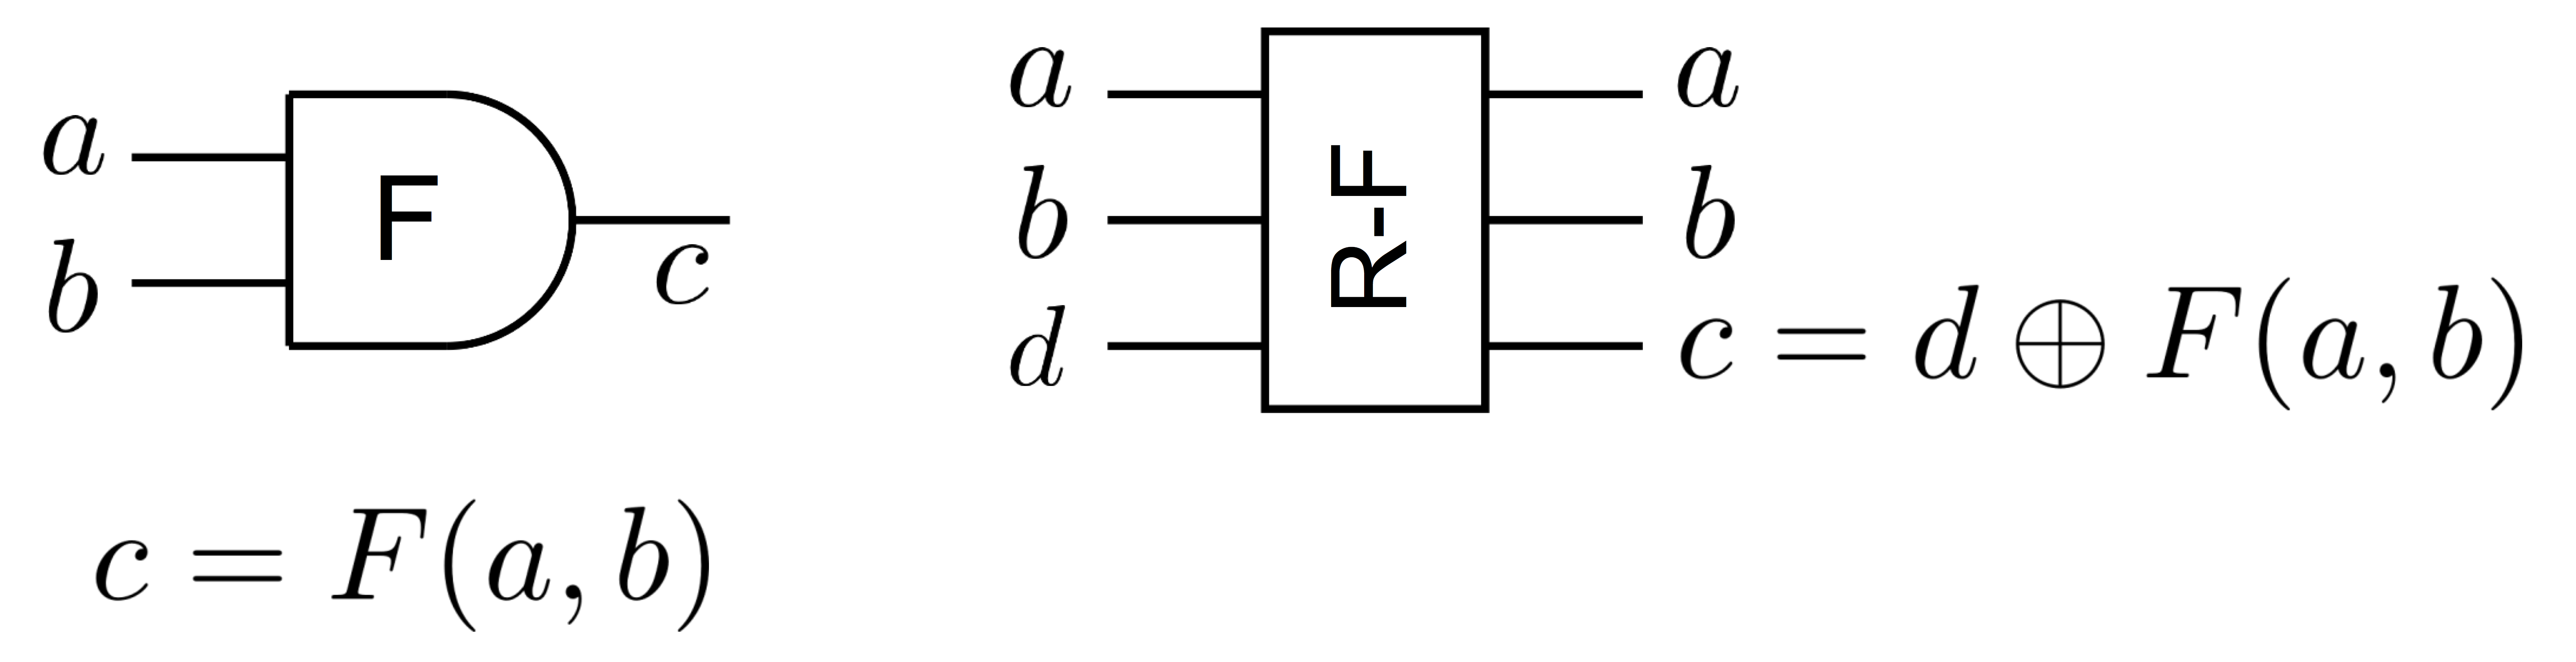
\includegraphics{r-f-gate.png}

\emph{Figure 2: Reversible F (R-F) gate. (Source: ``Shor's Algorithm''})

    \hypertarget{quantum-circuit-for-modular-multiplication}{%
\subsubsection{Quantum Circuit for Modular
Multiplication}\label{quantum-circuit-for-modular-multiplication}}

~~~~The modular exponentiation function can be derived from a series of
modular multiplication functions. Let the modular multiplication
function be defined as \(f(x)=ax\pmod N\). If the integer results of
\(f(x)\) are stored as \(n\)-bit strings, then \(f(x)\) can be
implemented as a classical circuit \(U_a\) (unitary operator described
above) using 3-bit reversible classical gates with \(n\) inputs and
\(n\) outputs via the reversible gate transformation technique described
above (``Shor's Algorithm''). Since \(U_a\) is now composed completely
of reversible classical circuits, it can be called as a classical
subroutine from a quantum routine.

    \hypertarget{ibm-quantum-experience}{%
\subsubsection{IBM Quantum Experience}\label{ibm-quantum-experience}}

~~~~IBM has a platform called the IBM Quantum Experience which allows
curious computer scientists to experiment with quantum computing
concepts. IBM quantum hardware runs
\href{https://github.com/QISKit/openqasm}{OpenQASM} quantum assembly
code, but the web interface also features called ``Composer'' which
allows quantum and classical gates to be click-and-dragged onto a
virtual circuit diagram. IBM also has a Python SDK which allows
developers to implement and run quantum subroutines from within Python
code, either on a local quantum simulator, an IBM Quantum Experience
simulator, or on real IBM quantum hardware.

A basic, crude implementation of Shor's algorithm can be found below; if
running in a Jupyter Notebook, it can be run interactively. The full
Python script can be found in the appendix.

    \begin{Verbatim}[commandchars=\\\{\}]
{\color{incolor}In [{\color{incolor}8}]:} \PY{c+c1}{\PYZsh{} \PYZpc{}load QuantumProgramRunner.py}
        \PY{c+c1}{\PYZsh{}!/usr/bin/env python3}
        \PY{k+kn}{from} \PY{n+nn}{Runner} \PY{k}{import} \PY{n}{run}
        
        \PY{k}{if} \PY{n+nv+vm}{\PYZus{}\PYZus{}name\PYZus{}\PYZus{}} \PY{o}{==} \PY{l+s+s2}{\PYZdq{}}\PY{l+s+s2}{\PYZus{}\PYZus{}main\PYZus{}\PYZus{}}\PY{l+s+s2}{\PYZdq{}}\PY{p}{:}
            \PY{k}{while} \PY{n}{run}\PY{p}{(}\PY{k+kc}{None}\PY{p}{)}\PY{p}{:}
                \PY{k}{pass}
\end{Verbatim}


    \begin{Verbatim}[commandchars=\\\{\}]






\textcolor{ansi-blue-intense}{Factorizing N=6378689{\ldots}}
\textcolor{ansi-yellow-intense}{Chose unlucky 'a' value, trying again with new 'a' value (18th try so far){\ldots}}
\textcolor{ansi-blue-intense}{Selected random value a=4854918 to find period.}
\textcolor{ansi-blue-intense}{Found common period between N=6378689 and a=4854918}
\textcolor{ansi-green-intense}{Took 18 guesses for 'a' value.             }
\textcolor{ansi-green-intense}{Found factors: 37 X 172397 = 6378689}
\textcolor{ansi-green-intense}{\textbf{Available programs:}}
\textcolor{ansi-blue-intense}{  1. find\_period: Takes two integers, a and N, and finds the period of the modular exponentiation function.}
\textcolor{ansi-blue-intense}{  2. factorize\_N: Takes an integer N and finds factors of N using Shor's algorithm.}
Select a program to run, or type 'exit' to quit.
> exit


    \end{Verbatim}

    \hypertarget{results}{%
\subsection{Results}\label{results}}

~~~~Because I could only get the QASM code to run properly on a quantum
simulator, and not real quantum hardware at IBM, I was unable to get
valid or usable results from my attempted benchmarking. The test data,
results, and graphs I generated, as well as the Python scripts used to
generate them, can be found in the appendix.

The time complexity of integer factorization and Shor's algorithm is a
function of the number of digits \(d\). The brute force solution for an
integer \(N\) simply iterates through prime numbers \(p\) up to
\(\sqrt N\) and checks if \(N\pmod p\stackrel{?}{=} 0\). A more
efficient solution, known as the quadratic sieve technique, searches for
two integers \(a, b\) such that \((a^2-b^2) \mod N\stackrel{?}{=} 0\);
this method has a runtime bounded by \(O(\sqrt d)\) where \(d\) is the
number of digits in \(N\). The most efficient known classical algorithm,
the general number field sieve achieves a complexity of \(O(d^{1/3})\).
Shor's algorithm achieves a time complexity \emph{polynomial} in terms
of \(d\) (``Shor's Algorithm'').

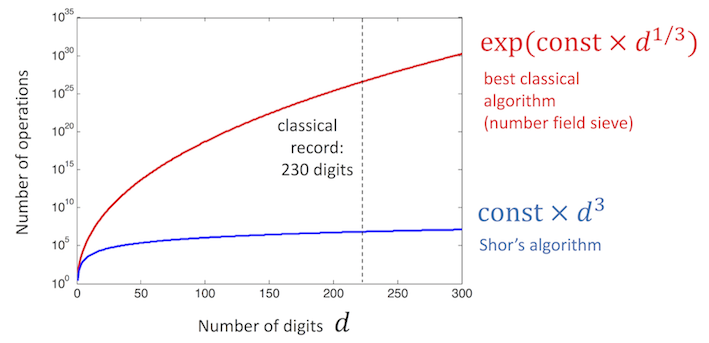
\includegraphics{shor-vs-classical.png}

\emph{Figure 3: Shor's algorithm vs.~the general number sieve algorithm.
(Source: ``Shor's Algorithm'')}

    \hypertarget{extensions}{%
\subsection{Extensions}\label{extensions}}

~~~~To date, Shor's algorithm is the only known algorithm for prime
factorization of large integers in polynomial time. On classical
computers, the Sieve of Eratosthenes can be used to find prime factors
of integers in \(O(nlg(lg(n)))\) time (\emph{Sorenson 1990}). Despite
being published in 1995, Shor's algorithm is still at the bleeding edge
of prime factorization algorithms and can be shown to have a time
complexity of
\(O((lg\hspace{1pt}n)^2(lg\hspace{1pt}lg\hspace{1pt}n)(lg\hspace{1pt}lg\hspace{1pt}lg\hspace{1pt}n))\)
(\emph{Beckman et al.~1996}).

    \hypertarget{conclusion}{%
\subsection{Conclusion}\label{conclusion}}

~~~~Shor's algorithm is perhaps the most radical example of how quantum
computing has changed (and can continue to change) the set of problems
considered feasible. In the past, prime factorization was a problem
considered so infeasible that a significant portion of existing
cryptography infrastructure is based on this assumption; this means that
quantum computing technology, along with Shor's algorithm, could be used
to crack nearly any common encryption used today. Shor's algorithm is on
the bleeding edge of quantum computing; as quantum computing technology
has gained traction in recent years, it has been used as a sort of
litmus test for quantum computer viability. IBM first demonstrated a
simple implementation of Shor's algorithm on one of their early quantum
computers in 2001, factorizing the number 15 into its factors 3 and 5
(\emph{``IBM's Test-Tube Quantum Computer Makes History'' 2001}).
Significant progress has been made since 2001 in the realm of quantum
computing technology, and for this reason, its important to begin
considering it as an inevitability which will come to fruition sooner
rather than later.

    \hypertarget{works-cited}{%
\subsection{Works Cited}\label{works-cited}}

Beckman, David, Amalavoyal N. Chari, Srikrishna Devabhaktuni, and John
Preskill. 1996. ``Efficient Networks for Quantum Factoring.'' Cornell
University. https://{}arxiv.org/abs/quant-ph/9602016.

``Deutsch-Jozsa Algorithm.'' Documentation. \emph{IBM Q Experience
Documentation.}
https://{}quantumexperience.ng.bluemix.net/proxy/tutorial/full-user-guide/004-Quantum\_Algorithms/080-Deutsch-Jozsa\_Algorithm.html.

``IBM's Test-Tube Quantum Computer Makes History.'' 2001. \emph{IBM News
Room}. December 19.
https://{}www-03.ibm.com/press/us/en/pressrelease/965.wss.

``Quantum Phase Estimation.'' Documentation. \emph{IBM Q Experience
Documentation.}
https://{}quantumexperience.ng.bluemix.net/proxy/tutorial/full-user-guide/004-Quantum\_Algorithms/100-Quantum\_Phase\_Estimation.html.

``Shor's Algorithm.'' Documentation. \emph{IBM Q Experience
Documentation.}
https://{}quantumexperience.ng.bluemix.net/proxy/tutorial/full-user-guide/004-Quantum\_Algorithms/110-Shor's\_algorithm.html.

Sorenson, Jonathan. 1990. ``An Introduction to Prime Number Sieves.''
University of Wisconsin-Madison.
http://{}research.cs.wisc.edu/techreports/1990/TR909.pdf.

    \hypertarget{appendix}{%
\subsection{Appendix}\label{appendix}}

    \hypertarget{github}{%
\subsubsection{GitHub}\label{github}}

~~ https://github.com/mrjones2014/CS360-shors-algorithm

    \hypertarget{quantumcircuits.py}{%
\subsubsection{QuantumCircuits.py}\label{quantumcircuits.py}}

    \begin{Verbatim}[commandchars=\\\{\}]
{\color{incolor}In [{\color{incolor} }]:} \PY{k+kn}{from} \PY{n+nn}{qiskit} \PY{k}{import} \PY{n}{QuantumProgram}
        \PY{k+kn}{from} \PY{n+nn}{qiskit} \PY{k}{import} \PY{n}{QuantumCircuit}
        \PY{k+kn}{from} \PY{n+nn}{qiskit} \PY{k}{import} \PY{n}{QuantumRegister}
        \PY{k+kn}{from} \PY{n+nn}{qiskit} \PY{k}{import} \PY{n}{ClassicalRegister}
        \PY{k+kn}{from} \PY{n+nn}{pyspin}\PY{n+nn}{.}\PY{n+nn}{spin} \PY{k}{import} \PY{n}{make\PYZus{}spin}\PY{p}{,} \PY{n}{Default}
        \PY{k+kn}{from} \PY{n+nn}{IPython}\PY{n+nn}{.}\PY{n+nn}{display} \PY{k}{import} \PY{n}{clear\PYZus{}output}
        \PY{k+kn}{from} \PY{n+nn}{math} \PY{k}{import} \PY{n}{sqrt}\PY{p}{;} \PY{k+kn}{from} \PY{n+nn}{itertools} \PY{k}{import} \PY{n}{count}\PY{p}{,} \PY{n}{islice}
        \PY{k+kn}{from} \PY{n+nn}{qiskit} \PY{k}{import} \PY{n}{Result}
        \PY{k+kn}{import} \PY{n+nn}{PrintUtils}
        \PY{k+kn}{import} \PY{n+nn}{QConfig}
        \PY{k+kn}{import} \PY{n+nn}{random}
        \PY{k+kn}{import} \PY{n+nn}{math}
        
        \PY{k}{class} \PY{n+nc}{Circuits}\PY{p}{:}
            \PY{c+c1}{\PYZsh{} String constants for circuit names}
            \PY{n}{PERIOD} \PY{o}{=} \PY{l+s+s2}{\PYZdq{}}\PY{l+s+s2}{circuit\PYZus{}period}\PY{l+s+s2}{\PYZdq{}} \PY{c+c1}{\PYZsh{} find\PYZus{}period() quantum circuit}
        
        \PY{k}{class} \PY{n+nc}{QRegs}\PY{p}{:}
            \PY{c+c1}{\PYZsh{} String constants for quantum register names}
            \PY{n}{PERIOD} \PY{o}{=} \PY{l+s+s2}{\PYZdq{}}\PY{l+s+s2}{qreg\PYZus{}period}\PY{l+s+s2}{\PYZdq{}} \PY{c+c1}{\PYZsh{} find\PYZus{}period() quantum register}
        
        \PY{k}{class} \PY{n+nc}{CRegs}\PY{p}{:}
            \PY{c+c1}{\PYZsh{} String constants for classical register names}
            \PY{n}{PERIOD} \PY{o}{=} \PY{l+s+s2}{\PYZdq{}}\PY{l+s+s2}{creg\PYZus{}period}\PY{l+s+s2}{\PYZdq{}} \PY{c+c1}{\PYZsh{} find\PYZus{}period() classical register}
        
        \PY{k}{class} \PY{n+nc}{QuantumPrograms}\PY{p}{:}
            \PY{n}{PROGRAMS} \PY{o}{=} \PY{p}{\PYZob{}}
                \PY{l+s+s2}{\PYZdq{}}\PY{l+s+s2}{find\PYZus{}period}\PY{l+s+s2}{\PYZdq{}}\PY{p}{:} \PY{l+s+s2}{\PYZdq{}}\PY{l+s+s2}{Takes two integers, a and N, and finds the period of the modular exponentiation function.}\PY{l+s+s2}{\PYZdq{}}\PY{p}{,}
                \PY{l+s+s2}{\PYZdq{}}\PY{l+s+s2}{factorize\PYZus{}N}\PY{l+s+s2}{\PYZdq{}}\PY{p}{:} \PY{l+s+s2}{\PYZdq{}}\PY{l+s+s2}{Takes an integer N and finds factors of N using Shor}\PY{l+s+s2}{\PYZsq{}}\PY{l+s+s2}{s algorithm.}\PY{l+s+s2}{\PYZdq{}}
            \PY{p}{\PYZcb{}}
            \PY{l+s+sd}{\PYZdq{}\PYZdq{}\PYZdq{}}
        \PY{l+s+sd}{    A class containing quantum circuits used in Shor\PYZsq{}s algorithm.}
        \PY{l+s+sd}{    Constructor takes an instance of a QuantumProgram object from QISKit module}
        \PY{l+s+sd}{    in order to create the circuits/run code on the IBM Quantum Experience hardware.}
        \PY{l+s+sd}{    \PYZdq{}\PYZdq{}\PYZdq{}}
        
            \PY{k}{def} \PY{n+nf}{\PYZus{}\PYZus{}init\PYZus{}\PYZus{}}\PY{p}{(}\PY{n+nb+bp}{self}\PY{p}{,} \PY{n}{quantum\PYZus{}program}\PY{p}{:} \PY{n}{QuantumProgram}\PY{p}{,} \PY{n}{qconfig}\PY{p}{:} \PY{n}{QConfig}\PY{p}{)}\PY{p}{:}
                \PY{l+s+sd}{\PYZdq{}\PYZdq{}\PYZdq{}Store QuantumProgram instance in self.\PYZdq{}\PYZdq{}\PYZdq{}}
                \PY{n+nb+bp}{self}\PY{o}{.}\PY{n}{qp} \PY{o}{=} \PY{n}{quantum\PYZus{}program}
                \PY{n+nb+bp}{self}\PY{o}{.}\PY{n}{qconf} \PY{o}{=} \PY{n}{qconfig}
            
            \PY{k}{def} \PY{n+nf}{gcd}\PY{p}{(}\PY{n+nb+bp}{self}\PY{p}{,} \PY{n}{a}\PY{p}{,} \PY{n}{b}\PY{p}{)}\PY{p}{:}
                \PY{l+s+sd}{\PYZdq{}\PYZdq{}\PYZdq{}Find Greatest Common Divisor (GCD) using Euclid\PYZsq{}s algorithm\PYZdq{}\PYZdq{}\PYZdq{}}
                \PY{k}{while} \PY{n}{b} \PY{o}{!=} \PY{l+m+mi}{0}\PY{p}{:}
                    \PY{p}{(}\PY{n}{a}\PY{p}{,} \PY{n}{b}\PY{p}{)} \PY{o}{=} \PY{p}{(}\PY{n}{b}\PY{p}{,} \PY{n}{a} \PY{o}{\PYZpc{}} \PY{n}{b}\PY{p}{)}
                \PY{k}{return} \PY{n}{a}
            
            \PY{k}{def} \PY{n+nf}{isPrime}\PY{p}{(}\PY{n+nb+bp}{self}\PY{p}{,} \PY{n}{n}\PY{p}{)}\PY{p}{:}
                \PY{k}{return} \PY{n}{n} \PY{o}{\PYZgt{}} \PY{l+m+mi}{1} \PY{o+ow}{and} \PY{n+nb}{all}\PY{p}{(}\PY{n}{n}\PY{o}{\PYZpc{}}\PY{k}{i} for i in islice(count(2), int(sqrt(n)\PYZhy{}1)))
        
            \PY{k}{def} \PY{n+nf}{factorize\PYZus{}N}\PY{p}{(}\PY{n+nb+bp}{self}\PY{p}{,} \PY{n}{N}\PY{p}{,} \PY{n}{numRetries}\PY{o}{=}\PY{l+m+mi}{0}\PY{p}{)}\PY{p}{:}
                \PY{l+s+sd}{\PYZdq{}\PYZdq{}\PYZdq{}Factorize N using Shor\PYZsq{}s algorithm.\PYZdq{}\PYZdq{}\PYZdq{}}
                \PY{n}{PrintUtils}\PY{o}{.}\PY{n}{printInfo}\PY{p}{(}\PY{n}{f}\PY{l+s+s2}{\PYZdq{}}\PY{l+s+s2}{Factorizing N=}\PY{l+s+si}{\PYZob{}N\PYZcb{}}\PY{l+s+s2}{...}\PY{l+s+s2}{\PYZdq{}}\PY{p}{)}
                \PY{k}{if} \PY{n}{numRetries} \PY{o}{\PYZgt{}} \PY{l+m+mi}{0}\PY{p}{:}
                    \PY{n}{clear\PYZus{}output}\PY{p}{(}\PY{p}{)}
                    \PY{k}{if} \PY{n}{numRetries} \PY{o}{\PYZgt{}} \PY{l+m+mi}{1}\PY{p}{:}
                        \PY{n}{PrintUtils}\PY{o}{.}\PY{n}{delete\PYZus{}last\PYZus{}lines}\PY{p}{(}\PY{l+m+mi}{6}\PY{p}{)}
                    \PY{k}{else}\PY{p}{:}
                        \PY{n}{PrintUtils}\PY{o}{.}\PY{n}{delete\PYZus{}last\PYZus{}lines}\PY{p}{(}\PY{l+m+mi}{5}\PY{p}{)}
                    \PY{n}{PrintUtils}\PY{o}{.}\PY{n}{printInfo}\PY{p}{(}\PY{n}{f}\PY{l+s+s2}{\PYZdq{}}\PY{l+s+s2}{Factorizing N=}\PY{l+s+si}{\PYZob{}N\PYZcb{}}\PY{l+s+s2}{...}\PY{l+s+s2}{\PYZdq{}}\PY{p}{)}
                    \PY{n}{PrintUtils}\PY{o}{.}\PY{n}{printWarning}\PY{p}{(}\PY{n}{f}\PY{l+s+s2}{\PYZdq{}}\PY{l+s+s2}{Chose unlucky }\PY{l+s+s2}{\PYZsq{}}\PY{l+s+s2}{a}\PY{l+s+s2}{\PYZsq{}}\PY{l+s+s2}{ value, trying again with new }\PY{l+s+s2}{\PYZsq{}}\PY{l+s+s2}{a}\PY{l+s+s2}{\PYZsq{}}\PY{l+s+s2}{ value (}\PY{l+s+s2}{\PYZob{}}\PY{l+s+s2}{PrintUtils.toOrdinal(numRetries + 1)\PYZcb{} try so far)...}\PY{l+s+s2}{\PYZdq{}}\PY{p}{)}
                
                \PY{c+c1}{\PYZsh{} Step 1: check if N is even; if so, simply divide by 2 and return the factors}
                \PY{k}{if} \PY{n}{N} \PY{o}{\PYZpc{}} \PY{l+m+mi}{2} \PY{o}{==} \PY{l+m+mi}{0}\PY{p}{:}
                    \PY{k}{return} \PY{p}{[}\PY{l+m+mi}{2}\PY{p}{,} \PY{n+nb}{int}\PY{p}{(}\PY{n}{N}\PY{o}{/}\PY{l+m+mi}{2}\PY{p}{)}\PY{p}{]}
                \PY{c+c1}{\PYZsh{} Step 2: choose random value for \PYZsq{}a\PYZsq{} between 2..(N\PYZhy{}1)}
                \PY{n}{a} \PY{o}{=} \PY{n}{random}\PY{o}{.}\PY{n}{randint}\PY{p}{(}\PY{l+m+mi}{2}\PY{p}{,} \PY{n}{N}\PY{o}{\PYZhy{}}\PY{l+m+mi}{1}\PY{p}{)}
                \PY{n}{PrintUtils}\PY{o}{.}\PY{n}{printInfo}\PY{p}{(}\PY{n}{f}\PY{l+s+s2}{\PYZdq{}}\PY{l+s+s2}{Selected random value a=}\PY{l+s+si}{\PYZob{}a\PYZcb{}}\PY{l+s+s2}{ to find period.}\PY{l+s+s2}{\PYZdq{}}\PY{p}{)}
                \PY{c+c1}{\PYZsh{} Step 3: determine if common period exists}
                \PY{n}{t} \PY{o}{=} \PY{n+nb+bp}{self}\PY{o}{.}\PY{n}{gcd}\PY{p}{(}\PY{n}{N}\PY{p}{,} \PY{n}{a}\PY{p}{)}
                \PY{k}{if} \PY{n}{t} \PY{o}{\PYZgt{}} \PY{l+m+mi}{1}\PY{p}{:}
                    \PY{n}{PrintUtils}\PY{o}{.}\PY{n}{printInfo}\PY{p}{(}\PY{n}{f}\PY{l+s+s2}{\PYZdq{}}\PY{l+s+s2}{Found common period between N=}\PY{l+s+si}{\PYZob{}N\PYZcb{}}\PY{l+s+s2}{ and a=}\PY{l+s+si}{\PYZob{}a\PYZcb{}}\PY{l+s+s2}{\PYZdq{}}\PY{p}{)}
                    \PY{n}{PrintUtils}\PY{o}{.}\PY{n}{printSuccess}\PY{p}{(}\PY{n}{f}\PY{l+s+s2}{\PYZdq{}}\PY{l+s+s2}{Took }\PY{l+s+s2}{\PYZob{}}\PY{l+s+s2}{numRetries + 1\PYZcb{} guesses for }\PY{l+s+s2}{\PYZsq{}}\PY{l+s+s2}{a}\PY{l+s+s2}{\PYZsq{}}\PY{l+s+s2}{ value.             }\PY{l+s+s2}{\PYZdq{}}\PY{p}{)}
                    \PY{k}{return} \PY{p}{[}\PY{n}{t}\PY{p}{,} \PY{n+nb}{int}\PY{p}{(}\PY{n}{N}\PY{o}{/}\PY{n}{t}\PY{p}{)}\PY{p}{]}
                \PY{c+c1}{\PYZsh{} Step 4: t=1, thus, N and a do not share common period. Find period using Shor\PYZsq{}s method.}
                \PY{n}{PrintUtils}\PY{o}{.}\PY{n}{printInfo}\PY{p}{(}\PY{l+s+s2}{\PYZdq{}}\PY{l+s+s2}{Using Shor}\PY{l+s+s2}{\PYZsq{}}\PY{l+s+s2}{s method to find period...}\PY{l+s+s2}{\PYZdq{}}\PY{p}{)}
                \PY{n}{r} \PY{o}{=} \PY{n+nb+bp}{self}\PY{o}{.}\PY{n}{find\PYZus{}period}\PY{p}{(}\PY{n}{a}\PY{p}{,} \PY{n}{N}\PY{p}{)}
                \PY{n}{factor1} \PY{o}{=} \PY{n+nb+bp}{self}\PY{o}{.}\PY{n}{gcd}\PY{p}{(}\PY{p}{(}\PY{n}{a}\PY{o}{*}\PY{o}{*}\PY{p}{(}\PY{n}{r}\PY{o}{/}\PY{l+m+mi}{2}\PY{p}{)}\PY{p}{)}\PY{o}{+}\PY{l+m+mi}{1}\PY{p}{,} \PY{n}{N}\PY{p}{)}
                \PY{k}{if} \PY{n}{factor1} \PY{o}{\PYZpc{}} \PY{n}{N} \PY{o}{==} \PY{l+m+mi}{0} \PY{o+ow}{or} \PY{n}{factor1} \PY{o}{==} \PY{l+m+mi}{1} \PY{o+ow}{or} \PY{n}{factor1} \PY{o}{==} \PY{n}{N} \PY{o+ow}{or} \PY{o+ow}{not}\PY{p}{(}\PY{n+nb+bp}{self}\PY{o}{.}\PY{n}{isPrime}\PY{p}{(}\PY{n}{factor1}\PY{p}{)}\PY{p}{)}\PY{p}{:}
                    \PY{k}{return} \PY{n+nb+bp}{self}\PY{o}{.}\PY{n}{factorize\PYZus{}N}\PY{p}{(}\PY{n}{N}\PY{p}{,} \PY{n}{numRetries} \PY{o}{+} \PY{l+m+mi}{1}\PY{p}{)}
                \PY{n}{factor2} \PY{o}{=} \PY{n}{N}\PY{o}{/}\PY{n}{factor1}
                \PY{k}{if} \PY{o+ow}{not} \PY{n+nb+bp}{self}\PY{o}{.}\PY{n}{isPrime}\PY{p}{(}\PY{n}{factor2}\PY{p}{)}\PY{p}{:}
                    \PY{k}{return} \PY{n+nb+bp}{self}\PY{o}{.}\PY{n}{factorize\PYZus{}N}\PY{p}{(}\PY{n}{N}\PY{p}{,} \PY{n}{numRetries} \PY{o}{+} \PY{l+m+mi}{1}\PY{p}{)}
                \PY{n}{PrintUtils}\PY{o}{.}\PY{n}{printSuccess}\PY{p}{(}\PY{n}{f}\PY{l+s+s2}{\PYZdq{}}\PY{l+s+s2}{Took }\PY{l+s+s2}{\PYZob{}}\PY{l+s+s2}{numRetries + 1\PYZcb{} guesses for }\PY{l+s+s2}{\PYZsq{}}\PY{l+s+s2}{a}\PY{l+s+s2}{\PYZsq{}}\PY{l+s+s2}{ value.             }\PY{l+s+s2}{\PYZdq{}}\PY{p}{)}
                \PY{k}{return} \PY{p}{[}\PY{n+nb}{int}\PY{p}{(}\PY{n}{factor1}\PY{p}{)}\PY{p}{,} \PY{n+nb}{int}\PY{p}{(}\PY{n}{factor2}\PY{p}{)}\PY{p}{]}
            
            \PY{n+nd}{@make\PYZus{}spin}\PY{p}{(}\PY{n}{Default}\PY{p}{,} \PY{l+s+s2}{\PYZdq{}}\PY{l+s+s2}{Finding period using Shor}\PY{l+s+s2}{\PYZsq{}}\PY{l+s+s2}{s method...}\PY{l+s+s2}{\PYZdq{}}\PY{p}{,} \PY{l+s+s2}{\PYZdq{}}\PY{l+s+se}{\PYZbs{}r}\PY{l+s+s2}{                                                    }\PY{l+s+se}{\PYZbs{}n}\PY{l+s+s2}{\PYZdq{}}\PY{p}{)}
            \PY{k}{def} \PY{n+nf}{find\PYZus{}period}\PY{p}{(}\PY{n+nb+bp}{self}\PY{p}{,} \PY{n}{a}\PY{p}{,} \PY{n}{N}\PY{p}{)}\PY{p}{:}
                \PY{l+s+sd}{\PYZdq{}\PYZdq{}\PYZdq{}}
        \PY{l+s+sd}{        Find the period of the modular exponentiation function, }
        \PY{l+s+sd}{        i.e. find r where (a\PYZca{}x) \PYZpc{} N=(a\PYZca{}[x + r]) \PYZpc{} N where x is any integer.}
        \PY{l+s+sd}{        For example:}
        \PY{l+s+sd}{        (7\PYZca{}2) \PYZpc{} 15 = 4 \PYZpc{} 15 = 4}
        \PY{l+s+sd}{        (7\PYZca{}3) \PYZpc{} 15 = (4 * 7) \PYZpc{} 15 = 13 \PYZpc{} 15 = 13}
        \PY{l+s+sd}{        (7\PYZca{}4) \PYZpc{} 15 = (13 * 7) \PYZpc{} 15 = 91 \PYZpc{} 15 = 1}
        \PY{l+s+sd}{        Thus, for a=7 and N=15, the periodic sequence is  (7\PYZca{}x) \PYZpc{} 15 = (7\PYZca{}[x + 4]) \PYZpc{} 15 for any integer x;}
        \PY{l+s+sd}{        therefore, the period for the modular exponentiation function for a=7 and N=15 is r=4.}
        \PY{l+s+sd}{        Returns a tuple containing the value of r and the number of iterations required to find r,}
        \PY{l+s+sd}{        (r, iterCount)}
        \PY{l+s+sd}{        \PYZdq{}\PYZdq{}\PYZdq{}}
                \PY{n+nb+bp}{self}\PY{o}{.}\PY{n}{create\PYZus{}modular\PYZus{}multiplication\PYZus{}circuit}\PY{p}{(}\PY{p}{)}
                \PY{n}{iterCount} \PY{o}{=} \PY{l+m+mi}{0}
                \PY{n}{r} \PY{o}{=} \PY{n}{math}\PY{o}{.}\PY{n}{inf} \PY{c+c1}{\PYZsh{} initialize r to infinity }
                \PY{k}{while} \PY{o+ow}{not} \PY{p}{(}\PY{p}{(}\PY{n}{r}\PY{o}{\PYZpc{}}\PY{k}{2} == 0) and (((a**(r/2))+1)\PYZpc{}N != 0) and (r != 0) and (r != 8)):
                    \PY{n}{iterCount} \PY{o}{+}\PY{o}{=} \PY{l+m+mi}{1}
                    \PY{n}{result}\PY{p}{:} \PY{n}{Result} \PY{o}{=} \PY{n+nb+bp}{self}\PY{o}{.}\PY{n}{qp}\PY{o}{.}\PY{n}{execute}\PY{p}{(}\PY{p}{[}\PY{n}{Circuits}\PY{o}{.}\PY{n}{PERIOD}\PY{p}{]}\PY{p}{,} \PY{n}{backend}\PY{o}{=}\PY{n+nb+bp}{self}\PY{o}{.}\PY{n}{qconf}\PY{o}{.}\PY{n}{backend}\PY{p}{,} \PY{n}{shots}\PY{o}{=}\PY{n+nb+bp}{self}\PY{o}{.}\PY{n}{qconf}\PY{o}{.}\PY{n}{shots}\PY{p}{,} \PY{n}{timeout}\PY{o}{=}\PY{n+nb+bp}{self}\PY{o}{.}\PY{n}{qconf}\PY{o}{.}\PY{n}{timeout}\PY{p}{)}
                    \PY{c+c1}{\PYZsh{} print(result)}
                    \PY{n}{data} \PY{o}{=} \PY{n}{result}\PY{o}{.}\PY{n}{get\PYZus{}counts}\PY{p}{(}\PY{n}{Circuits}\PY{o}{.}\PY{n}{PERIOD}\PY{p}{)}
                    \PY{c+c1}{\PYZsh{} print(data)}
                    \PY{n}{data} \PY{o}{=} \PY{n+nb}{list}\PY{p}{(}\PY{n}{data}\PY{o}{.}\PY{n}{keys}\PY{p}{(}\PY{p}{)}\PY{p}{)}
                    \PY{c+c1}{\PYZsh{} print(data)}
                    \PY{n}{r} \PY{o}{=} \PY{n+nb}{int}\PY{p}{(}\PY{n}{data}\PY{p}{[}\PY{l+m+mi}{0}\PY{p}{]}\PY{p}{)}
                    \PY{c+c1}{\PYZsh{} print(r)}
                    \PY{n}{l} \PY{o}{=} \PY{n+nb+bp}{self}\PY{o}{.}\PY{n}{gcd}\PY{p}{(}\PY{l+m+mi}{2}\PY{o}{*}\PY{o}{*}\PY{l+m+mi}{3}\PY{p}{,} \PY{n}{r}\PY{p}{)}
                    \PY{c+c1}{\PYZsh{} print(l)}
                    \PY{n}{r} \PY{o}{=} \PY{n+nb}{int}\PY{p}{(}\PY{p}{(}\PY{l+m+mi}{2}\PY{o}{*}\PY{o}{*}\PY{l+m+mi}{3}\PY{p}{)}\PY{o}{/}\PY{n}{l}\PY{p}{)}
                    \PY{c+c1}{\PYZsh{} print(r)}
                \PY{k}{return} \PY{n}{r}
        
            \PY{k}{def} \PY{n+nf}{create\PYZus{}modular\PYZus{}multiplication\PYZus{}circuit}\PY{p}{(}\PY{n+nb+bp}{self}\PY{p}{)}\PY{p}{:}
                \PY{n}{qr} \PY{o}{=} \PY{n+nb+bp}{self}\PY{o}{.}\PY{n}{qp}\PY{o}{.}\PY{n}{create\PYZus{}quantum\PYZus{}register}\PY{p}{(}\PY{n}{QRegs}\PY{o}{.}\PY{n}{PERIOD}\PY{p}{,} \PY{l+m+mi}{5}\PY{p}{)}
                \PY{n}{cr} \PY{o}{=} \PY{n+nb+bp}{self}\PY{o}{.}\PY{n}{qp}\PY{o}{.}\PY{n}{create\PYZus{}classical\PYZus{}register}\PY{p}{(}\PY{n}{CRegs}\PY{o}{.}\PY{n}{PERIOD}\PY{p}{,} \PY{l+m+mi}{3}\PY{p}{)}
                \PY{n+nb+bp}{self}\PY{o}{.}\PY{n}{qp}\PY{o}{.}\PY{n}{create\PYZus{}circuit}\PY{p}{(}\PY{n}{Circuits}\PY{o}{.}\PY{n}{PERIOD}\PY{p}{,} \PY{p}{[}\PY{n}{qr}\PY{p}{]}\PY{p}{,} \PY{p}{[}\PY{n}{cr}\PY{p}{]}\PY{p}{)}
                \PY{c+c1}{\PYZsh{} re\PYZhy{}fetch circuit and registers by name }
                \PY{n}{circuit}\PY{p}{:} \PY{n}{QuantumCircuit}  \PY{o}{=} \PY{n+nb+bp}{self}\PY{o}{.}\PY{n}{qp}\PY{o}{.}\PY{n}{get\PYZus{}circuit}\PY{p}{(}\PY{n}{Circuits}\PY{o}{.}\PY{n}{PERIOD}\PY{p}{)}
                \PY{n}{qreg}\PY{p}{:} \PY{n}{QuantumRegister} \PY{o}{=} \PY{n+nb+bp}{self}\PY{o}{.}\PY{n}{qp}\PY{o}{.}\PY{n}{get\PYZus{}quantum\PYZus{}register}\PY{p}{(}\PY{n}{QRegs}\PY{o}{.}\PY{n}{PERIOD}\PY{p}{)}
                \PY{n}{creg}\PY{p}{:} \PY{n}{ClassicalRegister} \PY{o}{=} \PY{n+nb+bp}{self}\PY{o}{.}\PY{n}{qp}\PY{o}{.}\PY{n}{get\PYZus{}classical\PYZus{}register}\PY{p}{(}\PY{n}{CRegs}\PY{o}{.}\PY{n}{PERIOD}\PY{p}{)}
                
                \PY{c+c1}{\PYZsh{}\PYZsh{} Set up the quantum circuit}
                \PY{c+c1}{\PYZsh{} Initialize: set qreg[0] to |1\PYZgt{} and }
                \PY{c+c1}{\PYZsh{} create superposition on top 8 qbits}
                \PY{n}{circuit}\PY{o}{.}\PY{n}{x}\PY{p}{(}\PY{n}{qreg}\PY{p}{[}\PY{l+m+mi}{0}\PY{p}{]}\PY{p}{)}
        
                \PY{c+c1}{\PYZsh{}\PYZsh{} Step 1: apply a\PYZca{}4 \PYZpc{} N}
                \PY{n}{circuit}\PY{o}{.}\PY{n}{h}\PY{p}{(}\PY{n}{qreg}\PY{p}{[}\PY{l+m+mi}{2}\PY{p}{]}\PY{p}{)}
                \PY{c+c1}{\PYZsh{} Controlled Identity gate}
                \PY{n}{circuit}\PY{o}{.}\PY{n}{h}\PY{p}{(}\PY{n}{qreg}\PY{p}{[}\PY{l+m+mi}{2}\PY{p}{]}\PY{p}{)}
                \PY{n}{circuit}\PY{o}{.}\PY{n}{measure}\PY{p}{(}\PY{n}{qreg}\PY{p}{[}\PY{l+m+mi}{2}\PY{p}{]}\PY{p}{,} \PY{n}{creg}\PY{p}{[}\PY{l+m+mi}{0}\PY{p}{]}\PY{p}{)} \PY{c+c1}{\PYZsh{} store the result}
                \PY{c+c1}{\PYZsh{} Reinitialize to |0\PYZgt{}}
                \PY{n}{circuit}\PY{o}{.}\PY{n}{reset}\PY{p}{(}\PY{n}{qreg}\PY{p}{[}\PY{l+m+mi}{2}\PY{p}{]}\PY{p}{)}
                \PY{c+c1}{\PYZsh{}\PYZsh{} Step 2: apply a\PYZca{}2 \PYZpc{} N}
                \PY{n}{circuit}\PY{o}{.}\PY{n}{h}\PY{p}{(}\PY{n}{qreg}\PY{p}{[}\PY{l+m+mi}{2}\PY{p}{]}\PY{p}{)}
                \PY{c+c1}{\PYZsh{} Controlled Identity gate }
                \PY{k}{if} \PY{n}{creg}\PY{p}{[}\PY{l+m+mi}{0}\PY{p}{]} \PY{o}{==} \PY{l+m+mi}{1}\PY{p}{:}
                    \PY{n}{circuit}\PY{o}{.}\PY{n}{u1}\PY{p}{(}\PY{n}{math}\PY{o}{.}\PY{n}{pi}\PY{o}{/}\PY{l+m+mf}{2.0}\PY{p}{,} \PY{n}{qreg}\PY{p}{[}\PY{l+m+mi}{2}\PY{p}{]}\PY{p}{)}
                \PY{n}{circuit}\PY{o}{.}\PY{n}{h}\PY{p}{(}\PY{n}{qreg}\PY{p}{[}\PY{l+m+mi}{2}\PY{p}{]}\PY{p}{)}
                \PY{n}{circuit}\PY{o}{.}\PY{n}{measure}\PY{p}{(}\PY{n}{qreg}\PY{p}{[}\PY{l+m+mi}{2}\PY{p}{]}\PY{p}{,} \PY{n}{creg}\PY{p}{[}\PY{l+m+mi}{1}\PY{p}{]}\PY{p}{)} \PY{c+c1}{\PYZsh{} store the result}
                \PY{c+c1}{\PYZsh{} Reinitialize to |0\PYZgt{}}
                \PY{n}{circuit}\PY{o}{.}\PY{n}{reset}\PY{p}{(}\PY{n}{qreg}\PY{p}{[}\PY{l+m+mi}{2}\PY{p}{]}\PY{p}{)}
                \PY{c+c1}{\PYZsh{}\PYZsh{} step 3: apply a \PYZpc{} N}
                \PY{n}{circuit}\PY{o}{.}\PY{n}{h}\PY{p}{(}\PY{n}{qreg}\PY{p}{[}\PY{l+m+mi}{2}\PY{p}{]}\PY{p}{)}
                \PY{c+c1}{\PYZsh{} Controlled NOT (C\PYZhy{}NOT) gate in between remaining gates}
                \PY{n}{circuit}\PY{o}{.}\PY{n}{cx}\PY{p}{(}\PY{n}{qreg}\PY{p}{[}\PY{l+m+mi}{2}\PY{p}{]}\PY{p}{,} \PY{n}{qreg}\PY{p}{[}\PY{l+m+mi}{1}\PY{p}{]}\PY{p}{)}
                \PY{n}{circuit}\PY{o}{.}\PY{n}{cx}\PY{p}{(}\PY{n}{qreg}\PY{p}{[}\PY{l+m+mi}{2}\PY{p}{]}\PY{p}{,} \PY{n}{qreg}\PY{p}{[}\PY{l+m+mi}{4}\PY{p}{]}\PY{p}{)}
        
                \PY{c+c1}{\PYZsh{}\PYZsh{} Feed forward }
                \PY{k}{if} \PY{n}{creg}\PY{p}{[}\PY{l+m+mi}{1}\PY{p}{]} \PY{o}{==} \PY{l+m+mi}{1}\PY{p}{:}
                    \PY{n}{circuit}\PY{o}{.}\PY{n}{u1}\PY{p}{(}\PY{n}{math}\PY{o}{.}\PY{n}{pi}\PY{o}{/}\PY{l+m+mf}{2.0}\PY{p}{,} \PY{n}{qreg}\PY{p}{[}\PY{l+m+mi}{2}\PY{p}{]}\PY{p}{)}
                \PY{k}{if} \PY{n}{creg}\PY{p}{[}\PY{l+m+mi}{0}\PY{p}{]} \PY{o}{==} \PY{l+m+mi}{1}\PY{p}{:}
                    \PY{n}{circuit}\PY{o}{.}\PY{n}{u1}\PY{p}{(}\PY{n}{math}\PY{o}{.}\PY{n}{pi}\PY{o}{/}\PY{l+m+mf}{4.0}\PY{p}{,} \PY{n}{qreg}\PY{p}{[}\PY{l+m+mi}{2}\PY{p}{]}\PY{p}{)}
                \PY{n}{circuit}\PY{o}{.}\PY{n}{h}\PY{p}{(}\PY{n}{qreg}\PY{p}{[}\PY{l+m+mi}{2}\PY{p}{]}\PY{p}{)}
                \PY{n}{circuit}\PY{o}{.}\PY{n}{measure}\PY{p}{(}\PY{n}{qreg}\PY{p}{[}\PY{l+m+mi}{2}\PY{p}{]}\PY{p}{,} \PY{n}{creg}\PY{p}{[}\PY{l+m+mi}{2}\PY{p}{]}\PY{p}{)} \PY{c+c1}{\PYZsh{} store the result}
                \PY{c+c1}{\PYZsh{} print(circuit.qasm()) \PYZsh{} print QASM code}
\end{Verbatim}


    \hypertarget{qconfig.py}{%
\subsubsection{QConfig.py}\label{qconfig.py}}

    \begin{Verbatim}[commandchars=\\\{\}]
{\color{incolor}In [{\color{incolor} }]:} \PY{k}{class} \PY{n+nc}{QConfig}\PY{p}{:} 
            \PY{k}{def} \PY{n+nf}{\PYZus{}\PYZus{}init\PYZus{}\PYZus{}}\PY{p}{(}\PY{n+nb+bp}{self}\PY{p}{,} \PY{n}{backend}\PY{p}{,} \PY{n}{shots}\PY{p}{,} \PY{n}{timeout}\PY{p}{,} \PY{n}{program}\PY{o}{=}\PY{k+kc}{None}\PY{p}{)}\PY{p}{:}
                \PY{n+nb+bp}{self}\PY{o}{.}\PY{n}{backend} \PY{o}{=} \PY{n}{backend}
                \PY{n+nb+bp}{self}\PY{o}{.}\PY{n}{shots} \PY{o}{=} \PY{n}{shots}
                \PY{n+nb+bp}{self}\PY{o}{.}\PY{n}{timeout} \PY{o}{=} \PY{n}{timeout}
                \PY{n+nb+bp}{self}\PY{o}{.}\PY{n}{program} \PY{o}{=} \PY{n}{program}
\end{Verbatim}


    \hypertarget{runner.py}{%
\subsubsection{Runner.py}\label{runner.py}}

    \begin{Verbatim}[commandchars=\\\{\}]
{\color{incolor}In [{\color{incolor} }]:} \PY{k+kn}{import} \PY{n+nn}{QuantumCircuits}
        \PY{k+kn}{import} \PY{n+nn}{ExperimentUtils}
        \PY{k+kn}{import} \PY{n+nn}{SignalUtils}
        \PY{k+kn}{import} \PY{n+nn}{PrintUtils}
        \PY{k+kn}{import} \PY{n+nn}{random}
        \PY{k+kn}{import} \PY{n+nn}{sys}
        
        \PY{k}{def} \PY{n+nf}{run}\PY{p}{(}\PY{n}{args}\PY{p}{)}\PY{p}{:}
            \PY{k}{return} \PY{n}{run\PYZus{}experiment}\PY{p}{(}\PY{n}{ExperimentUtils}\PY{o}{.}\PY{n}{setup\PYZus{}experiment}\PY{p}{(}\PY{n}{args}\PY{p}{)}\PY{p}{)}
        
        \PY{k}{def} \PY{n+nf}{run\PYZus{}experiment}\PY{p}{(}\PY{n}{experiment}\PY{p}{)}\PY{p}{:}
            \PY{n+nb}{print}\PY{p}{(}\PY{l+s+s2}{\PYZdq{}}\PY{l+s+s2}{\PYZdq{}}\PY{p}{)}
            \PY{n}{program} \PY{o}{=} \PY{n}{experiment}\PY{o}{.}\PY{n}{qconf}\PY{o}{.}\PY{n}{program}\PY{o}{.}\PY{n}{strip}\PY{p}{(}\PY{p}{)}
            \PY{n}{timeout} \PY{o}{=} \PY{n}{experiment}\PY{o}{.}\PY{n}{qconf}\PY{o}{.}\PY{n}{timeout}
            \PY{k}{if} \PY{n}{program} \PY{o}{==} \PY{l+s+s2}{\PYZdq{}}\PY{l+s+s2}{exit}\PY{l+s+s2}{\PYZdq{}}\PY{p}{:}
                \PY{k}{try}\PY{p}{:}
                    \PY{n}{sys}\PY{o}{.}\PY{n}{exit}\PY{p}{(}\PY{p}{)}
                \PY{k}{except}\PY{p}{:}
                    \PY{k}{try}\PY{p}{:}
                        \PY{n}{quit}\PY{p}{(}\PY{p}{)}
                    \PY{k}{except}\PY{p}{:}
                        \PY{k}{return}
            \PY{k}{elif} \PY{n}{program} \PY{o}{==} \PY{l+s+s2}{\PYZdq{}}\PY{l+s+s2}{find\PYZus{}period}\PY{l+s+s2}{\PYZdq{}}\PY{p}{:}
                \PY{n}{N} \PY{o}{=} \PY{n+nb}{int}\PY{p}{(}\PY{n+nb}{input}\PY{p}{(}\PY{l+s+s2}{\PYZdq{}}\PY{l+s+s2}{Enter a value for N:}\PY{l+s+se}{\PYZbs{}n}\PY{l+s+s2}{N = }\PY{l+s+s2}{\PYZdq{}}\PY{p}{)}\PY{p}{)}
                \PY{n}{a} \PY{o}{=} \PY{n+nb}{input}\PY{p}{(}\PY{l+s+s2}{\PYZdq{}}\PY{l+s+s2}{Enter a value for a (or type }\PY{l+s+s2}{\PYZsq{}}\PY{l+s+s2}{rand}\PY{l+s+s2}{\PYZsq{}}\PY{l+s+s2}{ for random value between 2..N\PYZhy{}1):}\PY{l+s+se}{\PYZbs{}n}\PY{l+s+s2}{a = }\PY{l+s+s2}{\PYZdq{}}\PY{p}{)}
                \PY{k}{if} \PY{n}{a} \PY{o}{==} \PY{l+s+s2}{\PYZdq{}}\PY{l+s+s2}{rand}\PY{l+s+s2}{\PYZdq{}}\PY{p}{:}
                    \PY{n}{a} \PY{o}{=} \PY{n}{random}\PY{o}{.}\PY{n}{randint}\PY{p}{(}\PY{l+m+mi}{2}\PY{p}{,} \PY{n}{N}\PY{o}{\PYZhy{}}\PY{l+m+mi}{1}\PY{p}{)}
                \PY{k}{else}\PY{p}{:}
                    \PY{n}{a} \PY{o}{=} \PY{n+nb}{int}\PY{p}{(}\PY{n}{a}\PY{p}{)}
                \PY{k}{def} \PY{n+nf}{run\PYZus{}expr}\PY{p}{(}\PY{p}{)}\PY{p}{:}
                    \PY{n}{r} \PY{o}{=} \PY{n}{experiment}\PY{o}{.}\PY{n}{find\PYZus{}period}\PY{p}{(}\PY{n}{a}\PY{p}{,} \PY{n}{N}\PY{p}{)}
                    \PY{n}{PrintUtils}\PY{o}{.}\PY{n}{printSuccess}\PY{p}{(}\PY{n}{f}\PY{l+s+s2}{\PYZdq{}}\PY{l+s+s2}{Found period r=}\PY{l+s+si}{\PYZob{}r\PYZcb{}}\PY{l+s+s2}{ for a=}\PY{l+s+si}{\PYZob{}a\PYZcb{}}\PY{l+s+s2}{ and N=}\PY{l+s+si}{\PYZob{}N\PYZcb{}}\PY{l+s+s2}{.}\PY{l+s+s2}{\PYZdq{}}\PY{p}{)}
                \PY{n}{SignalUtils}\PY{o}{.}\PY{n}{tryExecuteWithTimeout}\PY{p}{(}\PY{n}{run\PYZus{}expr}\PY{p}{,} \PY{n}{timeout}\PY{p}{,} \PY{n}{f}\PY{l+s+s2}{\PYZdq{}}\PY{l+s+se}{\PYZbs{}n}\PY{l+s+s2}{Failed to find period within timeout: }\PY{l+s+si}{\PYZob{}timeout\PYZcb{}}\PY{l+s+s2}{ seconds.}\PY{l+s+s2}{\PYZdq{}}\PY{p}{)}
                \PY{k}{return} \PY{k+kc}{True}
            \PY{k}{elif} \PY{n}{program} \PY{o}{==} \PY{l+s+s2}{\PYZdq{}}\PY{l+s+s2}{factorize\PYZus{}N}\PY{l+s+s2}{\PYZdq{}}\PY{p}{:}
                \PY{n}{N} \PY{o}{=} \PY{n+nb}{int}\PY{p}{(}\PY{n+nb}{input}\PY{p}{(}\PY{l+s+s2}{\PYZdq{}}\PY{l+s+s2}{Enter a value N to factorize:}\PY{l+s+se}{\PYZbs{}n}\PY{l+s+s2}{N = }\PY{l+s+s2}{\PYZdq{}}\PY{p}{)}\PY{p}{)}
                \PY{k}{def} \PY{n+nf}{run\PYZus{}expr}\PY{p}{(}\PY{p}{)}\PY{p}{:}
                    \PY{n}{factors} \PY{o}{=} \PY{n}{experiment}\PY{o}{.}\PY{n}{factorize\PYZus{}N}\PY{p}{(}\PY{n}{N}\PY{p}{)}
                    \PY{n}{PrintUtils}\PY{o}{.}\PY{n}{printSuccess}\PY{p}{(}\PY{n}{f}\PY{l+s+s2}{\PYZdq{}}\PY{l+s+s2}{Found factors: }\PY{l+s+si}{\PYZob{}factors[0]\PYZcb{}}\PY{l+s+s2}{ X }\PY{l+s+si}{\PYZob{}factors[1]\PYZcb{}}\PY{l+s+s2}{ = }\PY{l+s+si}{\PYZob{}N\PYZcb{}}\PY{l+s+s2}{\PYZdq{}}\PY{p}{)}
                \PY{n}{SignalUtils}\PY{o}{.}\PY{n}{tryExecuteWithTimeout}\PY{p}{(}\PY{n}{run\PYZus{}expr}\PY{p}{,} \PY{n}{timeout}\PY{p}{,} \PY{n}{f}\PY{l+s+s2}{\PYZdq{}}\PY{l+s+s2}{Failed to factorize }\PY{l+s+si}{\PYZob{}N\PYZcb{}}\PY{l+s+s2}{ within timeout: }\PY{l+s+si}{\PYZob{}timeout\PYZcb{}}\PY{l+s+s2}{ seconds.}\PY{l+s+s2}{\PYZdq{}}\PY{p}{)}
                \PY{k}{return} \PY{k+kc}{True}
            \PY{k}{else}\PY{p}{:} 
                \PY{n}{PrintUtils}\PY{o}{.}\PY{n}{printErr}\PY{p}{(}\PY{n}{f}\PY{l+s+s2}{\PYZdq{}}\PY{l+s+s2}{Invalid program }\PY{l+s+s2}{\PYZsq{}}\PY{l+s+si}{\PYZob{}program\PYZcb{}}\PY{l+s+s2}{\PYZsq{}}\PY{l+s+s2}{\PYZdq{}}\PY{p}{)}
\end{Verbatim}


    \hypertarget{experimentutils.py}{%
\subsubsection{ExperimentUtils.py}\label{experimentutils.py}}

    \begin{Verbatim}[commandchars=\\\{\}]
{\color{incolor}In [{\color{incolor} }]:} \PY{k+kn}{from} \PY{n+nn}{QuantumCircuits} \PY{k}{import} \PY{n}{QuantumPrograms}
        \PY{k+kn}{from} \PY{n+nn}{qiskit} \PY{k}{import} \PY{n}{QuantumProgram}
        \PY{k+kn}{from} \PY{n+nn}{QConfig} \PY{k}{import} \PY{n}{QConfig}
        \PY{k+kn}{import} \PY{n+nn}{PrintUtils}
        \PY{k+kn}{import} \PY{n+nn}{subprocess}
        \PY{k+kn}{import} \PY{n+nn}{os}
        
        \PY{k}{def} \PY{n+nf}{print\PYZus{}available\PYZus{}programs}\PY{p}{(}\PY{n}{programs}\PY{p}{)}\PY{p}{:}
            \PY{n}{PrintUtils}\PY{o}{.}\PY{n}{printHeader}\PY{p}{(}\PY{l+s+s2}{\PYZdq{}}\PY{l+s+s2}{Available programs:}\PY{l+s+s2}{\PYZdq{}}\PY{p}{)}
            \PY{n}{i} \PY{o}{=} \PY{l+m+mi}{1}
            \PY{k}{for} \PY{n}{progname} \PY{o+ow}{in} \PY{n}{programs}\PY{o}{.}\PY{n}{keys}\PY{p}{(}\PY{p}{)}\PY{p}{:}
                \PY{n}{PrintUtils}\PY{o}{.}\PY{n}{printInfo}\PY{p}{(}\PY{n}{f}\PY{l+s+s2}{\PYZdq{}}\PY{l+s+s2}{  }\PY{l+s+si}{\PYZob{}i\PYZcb{}}\PY{l+s+s2}{. }\PY{l+s+si}{\PYZob{}progname\PYZcb{}}\PY{l+s+s2}{: }\PY{l+s+si}{\PYZob{}programs[progname]\PYZcb{}}\PY{l+s+s2}{\PYZdq{}}\PY{p}{)}
                \PY{n}{i} \PY{o}{+}\PY{o}{=} \PY{l+m+mi}{1}
        
        \PY{k}{def} \PY{n+nf}{getParams}\PY{p}{(}\PY{p}{)}\PY{p}{:}
            \PY{n}{programs} \PY{o}{=} \PY{n}{QuantumPrograms}\PY{o}{.}\PY{n}{PROGRAMS}
        
            \PY{n}{backend} \PY{o}{=} \PY{l+s+s1}{\PYZsq{}}\PY{l+s+s1}{local\PYZus{}qasm\PYZus{}simulator}\PY{l+s+s1}{\PYZsq{}}
            \PY{n}{shots} \PY{o}{=} \PY{l+m+mi}{1024}
            \PY{n}{timeout} \PY{o}{=} \PY{l+m+mi}{120}
            \PY{n}{program} \PY{o}{=} \PY{k+kc}{None}
        
            \PY{n}{engine} \PY{o}{=} \PY{n}{QuantumProgram}\PY{p}{(}\PY{p}{)}
        
            \PY{k}{def} \PY{n+nf}{tryParseInt}\PY{p}{(}\PY{n}{value}\PY{p}{)}\PY{p}{:}
                \PY{k}{try}\PY{p}{:}
                    \PY{k}{return} \PY{n+nb}{int}\PY{p}{(}\PY{n}{value}\PY{p}{)}
                \PY{k}{except}\PY{p}{:}
                    \PY{k}{return} \PY{k+kc}{None}
            
            \PY{n}{print\PYZus{}available\PYZus{}programs}\PY{p}{(}\PY{n}{programs}\PY{p}{)}
            \PY{n}{program} \PY{o}{=} \PY{n+nb}{input}\PY{p}{(}\PY{l+s+s2}{\PYZdq{}}\PY{l+s+s2}{Select a program to run, or type }\PY{l+s+s2}{\PYZsq{}}\PY{l+s+s2}{exit}\PY{l+s+s2}{\PYZsq{}}\PY{l+s+s2}{ to quit.}\PY{l+s+se}{\PYZbs{}n}\PY{l+s+s2}{\PYZgt{} }\PY{l+s+s2}{\PYZdq{}}\PY{p}{)}\PY{o}{.}\PY{n}{strip}\PY{p}{(}\PY{p}{)}
            \PY{n}{progNum} \PY{o}{=} \PY{n}{tryParseInt}\PY{p}{(}\PY{n}{program}\PY{p}{)}
            \PY{k}{while} \PY{n}{program} \PY{o+ow}{not} \PY{o+ow}{in} \PY{n}{programs} \PY{o+ow}{and} \PY{n}{program} \PY{o}{!=} \PY{l+s+s2}{\PYZdq{}}\PY{l+s+s2}{exit}\PY{l+s+s2}{\PYZdq{}}\PY{p}{:}
                \PY{k}{if} \PY{n}{progNum} \PY{o+ow}{is} \PY{o+ow}{not} \PY{k+kc}{None}\PY{p}{:}
                    \PY{k}{if} \PY{n}{progNum} \PY{o}{\PYZgt{}} \PY{n+nb}{len}\PY{p}{(}\PY{n}{programs}\PY{p}{)}\PY{p}{:}
                        \PY{n}{PrintUtils}\PY{o}{.}\PY{n}{printErr}\PY{p}{(}\PY{n}{f}\PY{l+s+s2}{\PYZdq{}}\PY{l+s+s2}{Invalid program }\PY{l+s+s2}{\PYZsq{}}\PY{l+s+si}{\PYZob{}progNum\PYZcb{}}\PY{l+s+s2}{\PYZsq{}}\PY{l+s+s2}{\PYZdq{}}\PY{p}{)}
                    \PY{k}{else}\PY{p}{:}
                        \PY{n}{program} \PY{o}{=} \PY{n+nb}{list}\PY{p}{(}\PY{n}{programs}\PY{o}{.}\PY{n}{keys}\PY{p}{(}\PY{p}{)}\PY{p}{)}\PY{p}{[}\PY{n}{progNum} \PY{o}{\PYZhy{}} \PY{l+m+mi}{1}\PY{p}{]}
                        \PY{k}{break}
                \PY{k}{else}\PY{p}{:}
                    \PY{n}{PrintUtils}\PY{o}{.}\PY{n}{printErr}\PY{p}{(}\PY{n}{f}\PY{l+s+s2}{\PYZdq{}}\PY{l+s+s2}{Invalid program }\PY{l+s+s2}{\PYZsq{}}\PY{l+s+si}{\PYZob{}program\PYZcb{}}\PY{l+s+s2}{\PYZsq{}}\PY{l+s+s2}{\PYZdq{}}\PY{p}{)}
                \PY{n}{print\PYZus{}available\PYZus{}programs}\PY{p}{(}\PY{n}{programs}\PY{p}{)}
                \PY{n}{program} \PY{o}{=} \PY{n+nb}{input}\PY{p}{(}\PY{l+s+s2}{\PYZdq{}}\PY{l+s+s2}{Run which program?}\PY{l+s+se}{\PYZbs{}n}\PY{l+s+s2}{\PYZgt{} }\PY{l+s+s2}{\PYZdq{}}\PY{p}{)}\PY{o}{.}\PY{n}{strip}\PY{p}{(}\PY{p}{)}
                \PY{n}{progNum} \PY{o}{=} \PY{n}{tryParseInt}\PY{p}{(}\PY{n}{program}\PY{p}{)}
            \PY{k}{return} \PY{n}{QuantumPrograms}\PY{p}{(}\PY{n}{engine}\PY{p}{,} \PY{n}{QConfig}\PY{p}{(}\PY{n}{backend}\PY{p}{,} \PY{n}{shots}\PY{p}{,} \PY{n}{timeout}\PY{p}{,} \PY{n}{program}\PY{p}{)}\PY{p}{)}
        
        \PY{k}{def} \PY{n+nf}{setup\PYZus{}experiment}\PY{p}{(}\PY{n}{args}\PY{p}{)}\PY{p}{:}
            \PY{k}{if} \PY{n}{args} \PY{o+ow}{is} \PY{k+kc}{None}\PY{p}{:}
                \PY{k}{return} \PY{n}{getParams}\PY{p}{(}\PY{p}{)}
            \PY{k}{else}\PY{p}{:}
                \PY{n}{programs} \PY{o}{=} \PY{n}{QuantumPrograms}\PY{o}{.}\PY{n}{PROGRAMS}
        
                \PY{n}{apiToken} \PY{o}{=} \PY{k+kc}{None}
                \PY{n}{backend} \PY{o}{=} \PY{k+kc}{None}
                \PY{n}{shots} \PY{o}{=} \PY{k+kc}{None}
                \PY{n}{timeout} \PY{o}{=} \PY{k+kc}{None}
                \PY{n}{program} \PY{o}{=} \PY{k+kc}{None}
        
                \PY{c+c1}{\PYZsh{} get API token}
                \PY{k}{if} \PY{n}{args}\PY{o}{.}\PY{n}{apitoken} \PY{o+ow}{is} \PY{k+kc}{None}\PY{p}{:}
                    \PY{k}{try}\PY{p}{:}
                        \PY{n}{apiToken} \PY{o}{=} \PY{n+nb}{open}\PY{p}{(}\PY{l+s+s2}{\PYZdq{}}\PY{l+s+s2}{./.qiskit\PYZus{}api\PYZus{}token}\PY{l+s+s2}{\PYZdq{}}\PY{p}{,} \PY{l+s+s2}{\PYZdq{}}\PY{l+s+s2}{r}\PY{l+s+s2}{\PYZdq{}}\PY{p}{)}\PY{o}{.}\PY{n}{read}\PY{p}{(}\PY{p}{)}
                    \PY{k}{except}\PY{p}{:}
                        \PY{n}{apiToken} \PY{o}{=} \PY{n+nb}{input}\PY{p}{(}\PY{l+s+s2}{\PYZdq{}}\PY{l+s+s2}{Enter your IBM Quantum Experience API token: }\PY{l+s+se}{\PYZbs{}n}\PY{l+s+s2}{\PYZgt{} }\PY{l+s+s2}{\PYZdq{}}\PY{p}{)}
                \PY{k}{else}\PY{p}{:} 
                    \PY{n}{apiToken} \PY{o}{=} \PY{n}{args}\PY{o}{.}\PY{n}{apitoken}
                
                \PY{n}{engine} \PY{o}{=} \PY{n}{QuantumProgram}\PY{p}{(}\PY{p}{)}
                \PY{n}{engine}\PY{o}{.}\PY{n}{set\PYZus{}api}\PY{p}{(}\PY{n}{apiToken}\PY{p}{,} \PY{l+s+s1}{\PYZsq{}}\PY{l+s+s1}{https://quantumexperience.ng.bluemix.net/api}\PY{l+s+s1}{\PYZsq{}}\PY{p}{)}
        
                \PY{c+c1}{\PYZsh{} get backend}
                \PY{n}{backends} \PY{o}{=} \PY{n}{get\PYZus{}backend\PYZus{}dict}\PY{p}{(}\PY{n}{engine}\PY{o}{.}\PY{n}{available\PYZus{}backends}\PY{p}{(}\PY{p}{)}\PY{p}{)}
                \PY{k}{if} \PY{n}{args}\PY{o}{.}\PY{n}{backend} \PY{o+ow}{is} \PY{k+kc}{None}\PY{p}{:}
                    \PY{n}{PrintUtils}\PY{o}{.}\PY{n}{printHeader}\PY{p}{(}\PY{l+s+s2}{\PYZdq{}}\PY{l+s+s2}{Available backends:}\PY{l+s+s2}{\PYZdq{}}\PY{p}{)}
                    \PY{k}{for} \PY{n}{key}\PY{p}{,} \PY{n}{value} \PY{o+ow}{in} \PY{n}{backends}\PY{o}{.}\PY{n}{items}\PY{p}{(}\PY{p}{)}\PY{p}{:}
                        \PY{n}{PrintUtils}\PY{o}{.}\PY{n}{printInfo}\PY{p}{(}\PY{n}{f}\PY{l+s+s2}{\PYZdq{}}\PY{l+s+s2}{  }\PY{l+s+si}{\PYZob{}key\PYZcb{}}\PY{l+s+s2}{: }\PY{l+s+si}{\PYZob{}value\PYZcb{}}\PY{l+s+s2}{\PYZdq{}}\PY{p}{)}
                    \PY{n}{backend} \PY{o}{=} \PY{n}{get\PYZus{}backend}\PY{p}{(}\PY{n}{backends}\PY{p}{[}\PY{n+nb}{int}\PY{p}{(}\PY{n+nb}{input}\PY{p}{(}\PY{l+s+s2}{\PYZdq{}}\PY{l+s+s2}{Run on which backend?}\PY{l+s+se}{\PYZbs{}n}\PY{l+s+s2}{\PYZgt{} }\PY{l+s+s2}{\PYZdq{}}\PY{p}{)}\PY{p}{)}\PY{p}{]}\PY{p}{,} \PY{n}{backends}\PY{p}{)}
                \PY{k}{else}\PY{p}{:}
                    \PY{k}{if} \PY{n}{args}\PY{o}{.}\PY{n}{backend} \PY{o+ow}{in} \PY{n}{backends}\PY{o}{.}\PY{n}{values}\PY{p}{(}\PY{p}{)}\PY{p}{:}
                        \PY{n}{backend} \PY{o}{=} \PY{n}{args}\PY{o}{.}\PY{n}{backend}
                    \PY{k}{elif} \PY{n+nb}{int}\PY{p}{(}\PY{n}{args}\PY{o}{.}\PY{n}{backend}\PY{p}{)} \PY{o+ow}{in} \PY{n}{backends}\PY{o}{.}\PY{n}{keys}\PY{p}{(}\PY{p}{)}\PY{p}{:}
                        \PY{n}{backend} \PY{o}{=} \PY{n}{backends}\PY{p}{[}\PY{n+nb}{int}\PY{p}{(}\PY{n}{args}\PY{o}{.}\PY{n}{backend}\PY{p}{)}\PY{p}{]}
                    \PY{k}{else}\PY{p}{:} 
                        \PY{k}{raise} \PY{n+ne}{ValueError}\PY{p}{(}\PY{n}{f}\PY{l+s+s2}{\PYZdq{}}\PY{l+s+s2}{Invalid backend: }\PY{l+s+s2}{\PYZsq{}}\PY{l+s+si}{\PYZob{}args.backend\PYZcb{}}\PY{l+s+s2}{\PYZsq{}}\PY{l+s+s2}{\PYZdq{}}\PY{p}{)}
                
                \PY{c+c1}{\PYZsh{} set shots default value}
                \PY{k}{if} \PY{n}{args}\PY{o}{.}\PY{n}{shots} \PY{o+ow}{is} \PY{k+kc}{None}\PY{p}{:}
                    \PY{n}{shots} \PY{o}{=} \PY{l+m+mi}{1024}
                \PY{k}{else}\PY{p}{:}
                    \PY{n}{shots} \PY{o}{=} \PY{n+nb}{int}\PY{p}{(}\PY{n}{args}\PY{o}{.}\PY{n}{shots}\PY{p}{)}
                
                \PY{c+c1}{\PYZsh{} set timeout default value}
                \PY{k}{if} \PY{n}{args}\PY{o}{.}\PY{n}{timeout} \PY{o+ow}{is} \PY{k+kc}{None}\PY{p}{:}
                    \PY{n}{timeout} \PY{o}{=} \PY{l+m+mi}{120}
                \PY{k}{else}\PY{p}{:}
                    \PY{n}{timeout} \PY{o}{=} \PY{n+nb}{int}\PY{p}{(}\PY{n}{args}\PY{o}{.}\PY{n}{timeout}\PY{p}{)}
        
                \PY{c+c1}{\PYZsh{} validate program}
                \PY{k}{if} \PY{n}{args}\PY{o}{.}\PY{n}{program} \PY{o+ow}{is} \PY{k+kc}{None}\PY{p}{:}
                    \PY{n}{print\PYZus{}available\PYZus{}programs}\PY{p}{(}\PY{n}{programs}\PY{p}{)}
                    \PY{n}{program} \PY{o}{=} \PY{n+nb}{input}\PY{p}{(}\PY{l+s+s2}{\PYZdq{}}\PY{l+s+s2}{Run which program?}\PY{l+s+se}{\PYZbs{}n}\PY{l+s+s2}{\PYZgt{} }\PY{l+s+s2}{\PYZdq{}}\PY{p}{)}
                    \PY{k}{while} \PY{n}{program} \PY{o+ow}{not} \PY{o+ow}{in} \PY{n}{programs}\PY{p}{:}
                        \PY{n}{PrintUtils}\PY{o}{.}\PY{n}{printErr}\PY{p}{(}\PY{n}{f}\PY{l+s+s2}{\PYZdq{}}\PY{l+s+s2}{Invalid program }\PY{l+s+s2}{\PYZsq{}}\PY{l+s+si}{\PYZob{}program\PYZcb{}}\PY{l+s+s2}{\PYZsq{}}\PY{l+s+s2}{\PYZdq{}}\PY{p}{)}
                        \PY{n}{print\PYZus{}available\PYZus{}programs}\PY{p}{(}\PY{n}{programs}\PY{p}{)}
                        \PY{n}{program} \PY{o}{=} \PY{n+nb}{input}\PY{p}{(}\PY{l+s+s2}{\PYZdq{}}\PY{l+s+s2}{Run which program?}\PY{l+s+se}{\PYZbs{}n}\PY{l+s+s2}{\PYZgt{} }\PY{l+s+s2}{\PYZdq{}}\PY{p}{)}
                \PY{k}{else}\PY{p}{:}
                    \PY{k}{if} \PY{n}{args}\PY{o}{.}\PY{n}{program} \PY{o+ow}{not} \PY{o+ow}{in} \PY{n}{programs}\PY{o}{.}\PY{n}{keys}\PY{p}{(}\PY{p}{)}\PY{p}{:}
                        \PY{k}{raise} \PY{n+ne}{ValueError}\PY{p}{(}\PY{n}{f}\PY{l+s+s2}{\PYZdq{}}\PY{l+s+s2}{Invalid program }\PY{l+s+s2}{\PYZsq{}}\PY{l+s+si}{\PYZob{}args.program\PYZcb{}}\PY{l+s+s2}{\PYZsq{}}\PY{l+s+s2}{\PYZdq{}}\PY{p}{)}
                    \PY{k}{else}\PY{p}{:}
                        \PY{n}{program} \PY{o}{=} \PY{n}{args}\PY{o}{.}\PY{n}{program}
                
                \PY{k}{return} \PY{n}{QuantumPrograms}\PY{p}{(}\PY{n}{engine}\PY{p}{,} \PY{n}{QConfig}\PY{p}{(}\PY{n}{backend}\PY{p}{,} \PY{n}{shots}\PY{p}{,} \PY{n}{timeout}\PY{p}{,} \PY{n}{program}\PY{p}{)}\PY{p}{)}
        
        \PY{k}{def} \PY{n+nf}{get\PYZus{}backend\PYZus{}dict}\PY{p}{(}\PY{n}{backends}\PY{p}{)}\PY{p}{:}
            \PY{n+nb}{dict} \PY{o}{=} \PY{p}{\PYZob{}}\PY{p}{\PYZcb{}}
            \PY{n}{i} \PY{o}{=} \PY{l+m+mi}{1}
            \PY{c+c1}{\PYZsh{} ensure simulators are at top of list}
            \PY{k}{for} \PY{n}{b} \PY{o+ow}{in} \PY{n}{backends}\PY{p}{:}
                \PY{k}{if} \PY{l+s+s2}{\PYZdq{}}\PY{l+s+s2}{simulator}\PY{l+s+s2}{\PYZdq{}} \PY{o+ow}{in} \PY{n}{b}\PY{p}{:}
                    \PY{n+nb}{dict}\PY{p}{[}\PY{n}{i}\PY{p}{]} \PY{o}{=} \PY{n}{b}
                    \PY{n}{i} \PY{o}{+}\PY{o}{=} \PY{l+m+mi}{1}
            \PY{k}{for} \PY{n}{b} \PY{o+ow}{in} \PY{n}{backends}\PY{p}{:}
                \PY{k}{if} \PY{l+s+s2}{\PYZdq{}}\PY{l+s+s2}{simulator}\PY{l+s+s2}{\PYZdq{}} \PY{o+ow}{not} \PY{o+ow}{in} \PY{n}{b}\PY{p}{:}
                    \PY{n+nb}{dict}\PY{p}{[}\PY{n}{i}\PY{p}{]} \PY{o}{=} \PY{n}{b}
                    \PY{n}{i} \PY{o}{+}\PY{o}{=} \PY{l+m+mi}{1}
            \PY{k}{return} \PY{n+nb}{dict}
        
        \PY{k}{def} \PY{n+nf}{build\PYZus{}backend\PYZus{}dict}\PY{p}{(}\PY{n}{backends}\PY{p}{)}\PY{p}{:}
            \PY{n+nb}{dict} \PY{o}{=} \PY{p}{\PYZob{}}\PY{l+m+mi}{1}\PY{p}{:} \PY{l+s+s2}{\PYZdq{}}\PY{l+s+s2}{local\PYZus{}qasm\PYZus{}simulator}\PY{l+s+s2}{\PYZdq{}}\PY{p}{\PYZcb{}}
            \PY{n}{i} \PY{o}{=} \PY{l+m+mi}{2}
            \PY{c+c1}{\PYZsh{} ensure simulators are at top of list}
            \PY{k}{for} \PY{n}{b} \PY{o+ow}{in} \PY{n}{backends}\PY{p}{:}
                \PY{k}{if} \PY{l+s+s2}{\PYZdq{}}\PY{l+s+s2}{simulator}\PY{l+s+s2}{\PYZdq{}} \PY{o+ow}{in} \PY{n}{b}\PY{p}{[}\PY{l+s+s2}{\PYZdq{}}\PY{l+s+s2}{name}\PY{l+s+s2}{\PYZdq{}}\PY{p}{]}\PY{p}{:}
                    \PY{n+nb}{dict}\PY{p}{[}\PY{n}{i}\PY{p}{]} \PY{o}{=} \PY{n}{b}\PY{p}{[}\PY{l+s+s2}{\PYZdq{}}\PY{l+s+s2}{name}\PY{l+s+s2}{\PYZdq{}}\PY{p}{]}
                    \PY{n}{i} \PY{o}{+}\PY{o}{=} \PY{l+m+mi}{1}
            \PY{k}{for} \PY{n}{b} \PY{o+ow}{in} \PY{n}{backends}\PY{p}{:}
                \PY{k}{if} \PY{l+s+s2}{\PYZdq{}}\PY{l+s+s2}{simulator}\PY{l+s+s2}{\PYZdq{}} \PY{o+ow}{not} \PY{o+ow}{in} \PY{n}{b}\PY{p}{[}\PY{l+s+s2}{\PYZdq{}}\PY{l+s+s2}{name}\PY{l+s+s2}{\PYZdq{}}\PY{p}{]}\PY{p}{:}
                    \PY{n+nb}{dict}\PY{p}{[}\PY{n}{i}\PY{p}{]} \PY{o}{=} \PY{n}{b}\PY{p}{[}\PY{l+s+s2}{\PYZdq{}}\PY{l+s+s2}{name}\PY{l+s+s2}{\PYZdq{}}\PY{p}{]}
                    \PY{n}{i} \PY{o}{+}\PY{o}{=} \PY{l+m+mi}{1}
            \PY{k}{return} \PY{n+nb}{dict}
        
        \PY{k}{def} \PY{n+nf}{get\PYZus{}backend}\PY{p}{(}\PY{n}{i}\PY{p}{,} \PY{n}{available\PYZus{}backends}\PY{p}{)}\PY{p}{:}
            \PY{n}{backend} \PY{o}{=} \PY{k+kc}{None}
            \PY{k}{if} \PY{n}{i} \PY{o+ow}{in} \PY{n}{available\PYZus{}backends}\PY{o}{.}\PY{n}{keys}\PY{p}{(}\PY{p}{)}\PY{p}{:}
                \PY{k}{return} \PY{n}{available\PYZus{}backends}\PY{p}{[}\PY{n}{i}\PY{p}{]}
            \PY{k}{elif} \PY{n+nb}{str}\PY{p}{(}\PY{n}{i}\PY{p}{)} \PY{o+ow}{in} \PY{n}{available\PYZus{}backends}\PY{o}{.}\PY{n}{keys}\PY{p}{(}\PY{p}{)}\PY{p}{:}
                \PY{k}{return} \PY{n}{available\PYZus{}backends}\PY{p}{[}\PY{n+nb}{str}\PY{p}{(}\PY{n}{i}\PY{p}{)}\PY{p}{]}
            \PY{k}{elif} \PY{n+nb}{str}\PY{p}{(}\PY{n}{i}\PY{p}{)} \PY{o+ow}{in} \PY{n}{available\PYZus{}backends}\PY{o}{.}\PY{n}{values}\PY{p}{(}\PY{p}{)}\PY{p}{:}
                \PY{k}{return} \PY{n+nb}{str}\PY{p}{(}\PY{n}{i}\PY{p}{)}
            \PY{k}{else}\PY{p}{:}
                \PY{n}{PrintUtils}\PY{o}{.}\PY{n}{printErr}\PY{p}{(}\PY{n}{f}\PY{l+s+s2}{\PYZdq{}}\PY{l+s+s2}{Invalid backend }\PY{l+s+s2}{\PYZsq{}}\PY{l+s+si}{\PYZob{}backend\PYZcb{}}\PY{l+s+s2}{\PYZsq{}}\PY{l+s+s2}{, using default simulator...}\PY{l+s+s2}{\PYZdq{}}\PY{p}{)}
                \PY{k}{return} \PY{n+nb}{next}\PY{p}{(}\PY{n+nb}{iter}\PY{p}{(}\PY{n}{available\PYZus{}backends}\PY{o}{.}\PY{n}{values}\PY{p}{(}\PY{p}{)}\PY{p}{)}\PY{p}{)} \PY{c+c1}{\PYZsh{} first value in dict}
        
        \PY{k}{def} \PY{n+nf}{request\PYZus{}input\PYZus{}file}\PY{p}{(}\PY{p}{)}\PY{p}{:}
            \PY{n}{files} \PY{o}{=} \PY{p}{[}\PY{n}{i} \PY{k}{for} \PY{n}{i} \PY{o+ow}{in} \PY{n}{os}\PY{o}{.}\PY{n}{listdir}\PY{p}{(}\PY{l+s+s2}{\PYZdq{}}\PY{l+s+s2}{.}\PY{l+s+s2}{\PYZdq{}}\PY{p}{)} \PY{k}{if} \PY{n}{i}\PY{o}{.}\PY{n}{endswith}\PY{p}{(}\PY{l+s+s2}{\PYZdq{}}\PY{l+s+s2}{.qasm}\PY{l+s+s2}{\PYZdq{}}\PY{p}{)}\PY{p}{]}
            \PY{n}{PrintUtils}\PY{o}{.}\PY{n}{printHeader}\PY{p}{(}\PY{l+s+s2}{\PYZdq{}}\PY{l+s+s2}{QASM files found in current directory: }\PY{l+s+s2}{\PYZdq{}}\PY{p}{)}
            \PY{k}{for} \PY{n}{i} \PY{o+ow}{in} \PY{n}{files}\PY{p}{:}
                \PY{n}{PrintUtils}\PY{o}{.}\PY{n}{printInfo}\PY{p}{(}\PY{n}{f}\PY{l+s+s2}{\PYZdq{}}\PY{l+s+s2}{    ./}\PY{l+s+si}{\PYZob{}i\PYZcb{}}\PY{l+s+s2}{\PYZdq{}}\PY{p}{)}
            \PY{n}{file} \PY{o}{=} \PY{n}{subprocess}\PY{o}{.}\PY{n}{check\PYZus{}output}\PY{p}{(}\PY{l+s+s1}{\PYZsq{}}\PY{l+s+s1}{read \PYZhy{}e \PYZhy{}p }\PY{l+s+s1}{\PYZdq{}}\PY{l+s+s1}{Enter path to QASM file to run: }\PY{l+s+se}{\PYZbs{}n}\PY{l+s+s1}{\PYZgt{} }\PY{l+s+s1}{\PYZdq{}}\PY{l+s+s1}{ var ; echo \PYZdl{}var}\PY{l+s+s1}{\PYZsq{}}\PY{p}{,}\PY{n}{shell}\PY{o}{=}\PY{k+kc}{True}\PY{p}{)}\PY{o}{.}\PY{n}{rstrip}\PY{p}{(}\PY{p}{)}
            \PY{k}{return} \PY{n}{file}
\end{Verbatim}


    \hypertarget{signalutils.py}{%
\subsubsection{SignalUtils.py}\label{signalutils.py}}

    \begin{Verbatim}[commandchars=\\\{\}]
{\color{incolor}In [{\color{incolor} }]:} \PY{k+kn}{import} \PY{n+nn}{signal}
        \PY{k+kn}{import} \PY{n+nn}{PrintUtils}
        
        \PY{k}{class} \PY{n+nc}{TimeoutError}\PY{p}{(}\PY{n+ne}{Exception}\PY{p}{)}\PY{p}{:}
            \PY{k}{pass}
        
        \PY{k}{def} \PY{n+nf}{handler}\PY{p}{(}\PY{n}{signum}\PY{p}{,} \PY{n}{frame}\PY{p}{)}\PY{p}{:}
            \PY{k}{raise} \PY{n+ne}{TimeoutError}\PY{p}{(}\PY{p}{)}
        
        \PY{k}{def} \PY{n+nf}{tryExecuteWithTimeout}\PY{p}{(}\PY{n}{func}\PY{p}{,} \PY{n}{timeout}\PY{p}{,} \PY{n}{failMessage}\PY{p}{)}\PY{p}{:}
            \PY{n}{signal}\PY{o}{.}\PY{n}{signal}\PY{p}{(}\PY{n}{signal}\PY{o}{.}\PY{n}{SIGALRM}\PY{p}{,} \PY{n}{handler}\PY{p}{)}
            \PY{n}{signal}\PY{o}{.}\PY{n}{alarm}\PY{p}{(}\PY{n}{timeout}\PY{p}{)}
            \PY{k}{try}\PY{p}{:}
                \PY{n}{func}\PY{p}{(}\PY{p}{)}
            \PY{k}{except} \PY{n+ne}{TimeoutError}\PY{p}{:}
                \PY{n}{PrintUtils}\PY{o}{.}\PY{n}{printErr}\PY{p}{(}\PY{n}{failMessage}\PY{p}{)}
\end{Verbatim}


    \hypertarget{printutils.py}{%
\subsubsection{PrintUtils.py}\label{printutils.py}}

    \begin{Verbatim}[commandchars=\\\{\}]
{\color{incolor}In [{\color{incolor} }]:} \PY{k}{class} \PY{n+nc}{bcolors}\PY{p}{:}
            \PY{n}{OKBLUE} \PY{o}{=} \PY{l+s+s1}{\PYZsq{}}\PY{l+s+se}{\PYZbs{}033}\PY{l+s+s1}{[94m}\PY{l+s+s1}{\PYZsq{}}
            \PY{n}{OKGREEN} \PY{o}{=} \PY{l+s+s1}{\PYZsq{}}\PY{l+s+se}{\PYZbs{}033}\PY{l+s+s1}{[92m}\PY{l+s+s1}{\PYZsq{}}
            \PY{n}{WARNING} \PY{o}{=} \PY{l+s+s1}{\PYZsq{}}\PY{l+s+se}{\PYZbs{}033}\PY{l+s+s1}{[93m}\PY{l+s+s1}{\PYZsq{}}
            \PY{n}{FAIL} \PY{o}{=} \PY{l+s+s1}{\PYZsq{}}\PY{l+s+se}{\PYZbs{}033}\PY{l+s+s1}{[91m}\PY{l+s+s1}{\PYZsq{}}
            \PY{n}{ENDC} \PY{o}{=} \PY{l+s+s1}{\PYZsq{}}\PY{l+s+se}{\PYZbs{}033}\PY{l+s+s1}{[0m}\PY{l+s+s1}{\PYZsq{}}
            \PY{n}{BOLD} \PY{o}{=} \PY{l+s+s1}{\PYZsq{}}\PY{l+s+se}{\PYZbs{}033}\PY{l+s+s1}{[1m}\PY{l+s+s1}{\PYZsq{}}
            \PY{n}{UNDERLINE} \PY{o}{=} \PY{l+s+s1}{\PYZsq{}}\PY{l+s+se}{\PYZbs{}033}\PY{l+s+s1}{[4m}\PY{l+s+s1}{\PYZsq{}}
            \PY{n}{HEADER} \PY{o}{=} \PY{n}{BOLD} \PY{o}{+} \PY{n}{UNDERLINE} \PY{o}{+} \PY{n}{OKGREEN}
        
        \PY{k}{def} \PY{n+nf}{printErr}\PY{p}{(}\PY{n+nb}{str}\PY{p}{)}\PY{p}{:}
            \PY{n+nb}{print}\PY{p}{(}\PY{n}{f}\PY{l+s+s2}{\PYZdq{}}\PY{l+s+si}{\PYZob{}bcolors.FAIL\PYZcb{}}\PY{l+s+si}{\PYZob{}str\PYZcb{}}\PY{l+s+si}{\PYZob{}bcolors.ENDC\PYZcb{}}\PY{l+s+s2}{\PYZdq{}}\PY{p}{)}
        
        \PY{k}{def} \PY{n+nf}{printSuccess}\PY{p}{(}\PY{n+nb}{str}\PY{p}{)}\PY{p}{:}
            \PY{n+nb}{print}\PY{p}{(}\PY{n}{f}\PY{l+s+s2}{\PYZdq{}}\PY{l+s+si}{\PYZob{}bcolors.OKGREEN\PYZcb{}}\PY{l+s+si}{\PYZob{}str\PYZcb{}}\PY{l+s+si}{\PYZob{}bcolors.ENDC\PYZcb{}}\PY{l+s+s2}{\PYZdq{}}\PY{p}{)}
        
        \PY{k}{def} \PY{n+nf}{printInfo}\PY{p}{(}\PY{n+nb}{str}\PY{p}{)}\PY{p}{:}
            \PY{n+nb}{print}\PY{p}{(}\PY{n}{f}\PY{l+s+s2}{\PYZdq{}}\PY{l+s+si}{\PYZob{}bcolors.OKBLUE\PYZcb{}}\PY{l+s+si}{\PYZob{}str\PYZcb{}}\PY{l+s+si}{\PYZob{}bcolors.ENDC\PYZcb{}}\PY{l+s+s2}{\PYZdq{}}\PY{p}{)}
        
        \PY{k}{def} \PY{n+nf}{printWarning}\PY{p}{(}\PY{n+nb}{str}\PY{p}{)}\PY{p}{:}
            \PY{n+nb}{print}\PY{p}{(}\PY{n}{f}\PY{l+s+s2}{\PYZdq{}}\PY{l+s+si}{\PYZob{}bcolors.WARNING\PYZcb{}}\PY{l+s+si}{\PYZob{}str\PYZcb{}}\PY{l+s+si}{\PYZob{}bcolors.ENDC\PYZcb{}}\PY{l+s+s2}{\PYZdq{}}\PY{p}{)}
        
        \PY{k}{def} \PY{n+nf}{printHeader}\PY{p}{(}\PY{n+nb}{str}\PY{p}{)}\PY{p}{:}
            \PY{n+nb}{print}\PY{p}{(}\PY{n}{f}\PY{l+s+s2}{\PYZdq{}}\PY{l+s+si}{\PYZob{}bcolors.HEADER\PYZcb{}}\PY{l+s+si}{\PYZob{}str\PYZcb{}}\PY{l+s+si}{\PYZob{}bcolors.ENDC\PYZcb{}}\PY{l+s+s2}{\PYZdq{}}\PY{p}{)}
        
        \PY{k}{def} \PY{n+nf}{delete\PYZus{}last\PYZus{}lines}\PY{p}{(}\PY{n}{n}\PY{p}{)}\PY{p}{:}
            \PY{n}{CURSOR\PYZus{}UP\PYZus{}ONE} \PY{o}{=} \PY{l+s+s1}{\PYZsq{}}\PY{l+s+se}{\PYZbs{}x1b}\PY{l+s+s1}{[1A}\PY{l+s+s1}{\PYZsq{}}
            \PY{n}{ERASE\PYZus{}LINE} \PY{o}{=} \PY{l+s+s1}{\PYZsq{}}\PY{l+s+se}{\PYZbs{}x1b}\PY{l+s+s1}{[2K}\PY{l+s+s1}{\PYZsq{}}
            \PY{k}{for} \PY{n}{i} \PY{o+ow}{in} \PY{n+nb}{range}\PY{p}{(}\PY{l+m+mi}{0}\PY{p}{,} \PY{n}{n}\PY{p}{)}\PY{p}{:}
                \PY{n+nb}{print}\PY{p}{(}\PY{n}{CURSOR\PYZus{}UP\PYZus{}ONE}\PY{p}{,} \PY{n}{end}\PY{o}{=}\PY{l+s+s2}{\PYZdq{}}\PY{l+s+s2}{\PYZdq{}}\PY{p}{)}
            \PY{k}{for} \PY{n}{i} \PY{o+ow}{in} \PY{n+nb}{range}\PY{p}{(}\PY{l+m+mi}{0}\PY{p}{,} \PY{n}{n}\PY{p}{)}\PY{p}{:}
                \PY{n+nb}{print}\PY{p}{(}\PY{n}{ERASE\PYZus{}LINE}\PY{p}{)}
            \PY{k}{for} \PY{n}{i} \PY{o+ow}{in} \PY{n+nb}{range}\PY{p}{(}\PY{l+m+mi}{0}\PY{p}{,} \PY{n}{n}\PY{p}{)}\PY{p}{:}
                \PY{n+nb}{print}\PY{p}{(}\PY{n}{CURSOR\PYZus{}UP\PYZus{}ONE}\PY{p}{,} \PY{n}{end}\PY{o}{=}\PY{l+s+s2}{\PYZdq{}}\PY{l+s+s2}{\PYZdq{}}\PY{p}{)}
        
        \PY{k}{def} \PY{n+nf}{toOrdinal}\PY{p}{(}\PY{n}{n}\PY{p}{)}\PY{p}{:}
            \PY{k}{if} \PY{n}{n} \PY{o}{==} \PY{l+m+mi}{1}\PY{p}{:}
                \PY{k}{return} \PY{l+s+s2}{\PYZdq{}}\PY{l+s+s2}{1st}\PY{l+s+s2}{\PYZdq{}}
            \PY{k}{elif} \PY{n}{n} \PY{o}{==} \PY{l+m+mi}{2}\PY{p}{:}
                \PY{k}{return} \PY{l+s+s2}{\PYZdq{}}\PY{l+s+s2}{2nd}\PY{l+s+s2}{\PYZdq{}}
            \PY{k}{elif} \PY{n}{n} \PY{o}{==} \PY{l+m+mi}{3}\PY{p}{:}
                \PY{k}{return} \PY{l+s+s2}{\PYZdq{}}\PY{l+s+s2}{3rd}\PY{l+s+s2}{\PYZdq{}}
            \PY{k}{else}\PY{p}{:} 
                \PY{k}{return} \PY{n}{f}\PY{l+s+s2}{\PYZdq{}}\PY{l+s+si}{\PYZob{}n\PYZcb{}}\PY{l+s+s2}{th}\PY{l+s+s2}{\PYZdq{}}
\end{Verbatim}


    \hypertarget{benchmarkrunner.py}{%
\subsubsection{BenchmarkRunner.py}\label{benchmarkrunner.py}}

    \begin{Verbatim}[commandchars=\\\{\}]
{\color{incolor}In [{\color{incolor} }]:} \PY{c+ch}{\PYZsh{}!/usr/bin/env python3}
        
        \PY{k+kn}{from} \PY{n+nn}{QuantumCircuits} \PY{k}{import} \PY{n}{QuantumPrograms}
        \PY{k+kn}{from} \PY{n+nn}{qiskit} \PY{k}{import} \PY{n}{QuantumProgram}
        \PY{k+kn}{from} \PY{n+nn}{QConfig} \PY{k}{import} \PY{n}{QConfig}
        \PY{k+kn}{from} \PY{n+nn}{SignalUtils} \PY{k}{import} \PY{n}{tryExecuteWithTimeout}
        \PY{k+kn}{from} \PY{n+nn}{random} \PY{k}{import} \PY{n}{randint}
        \PY{k+kn}{import} \PY{n+nn}{time}
        \PY{k+kn}{import} \PY{n+nn}{sys}
        
        \PY{k}{def} \PY{n+nf}{setup\PYZus{}quantum\PYZus{}program}\PY{p}{(}\PY{p}{)}\PY{p}{:}
            \PY{n}{timeout} \PY{o}{=} \PY{l+m+mi}{210} \PY{c+c1}{\PYZsh{} 3.5 minutes}
            \PY{c+c1}{\PYZsh{} timeout = 80 \PYZsh{} for debugging}
            \PY{n}{shots} \PY{o}{=} \PY{l+m+mi}{1024}
            \PY{n}{backend} \PY{o}{=} \PY{l+s+s1}{\PYZsq{}}\PY{l+s+s1}{local\PYZus{}qasm\PYZus{}simulator}\PY{l+s+s1}{\PYZsq{}}
            \PY{n}{program} \PY{o}{=} \PY{l+s+s1}{\PYZsq{}}\PY{l+s+s1}{factorize\PYZus{}N}\PY{l+s+s1}{\PYZsq{}}
        
            \PY{n}{engine} \PY{o}{=} \PY{n}{QuantumProgram}\PY{p}{(}\PY{p}{)}
            \PY{n}{apiToken} \PY{o}{=} \PY{k+kc}{None}
            \PY{k}{try}\PY{p}{:}
                \PY{n}{apiToken} \PY{o}{=} \PY{n+nb}{open}\PY{p}{(}\PY{l+s+s2}{\PYZdq{}}\PY{l+s+s2}{./.qiskit\PYZus{}api\PYZus{}token}\PY{l+s+s2}{\PYZdq{}}\PY{p}{,} \PY{l+s+s2}{\PYZdq{}}\PY{l+s+s2}{r}\PY{l+s+s2}{\PYZdq{}}\PY{p}{)}\PY{o}{.}\PY{n}{read}\PY{p}{(}\PY{p}{)}
            \PY{k}{except}\PY{p}{:}
                \PY{n}{apiToken} \PY{o}{=} \PY{n+nb}{input}\PY{p}{(}\PY{l+s+s2}{\PYZdq{}}\PY{l+s+s2}{Enter your IBM Quantum Experience API token: }\PY{l+s+se}{\PYZbs{}n}\PY{l+s+s2}{\PYZgt{} }\PY{l+s+s2}{\PYZdq{}}\PY{p}{)}
        
            \PY{n}{engine}\PY{o}{.}\PY{n}{set\PYZus{}api}\PY{p}{(}\PY{n}{apiToken}\PY{p}{,} \PY{l+s+s1}{\PYZsq{}}\PY{l+s+s1}{https://quantumexperience.ng.bluemix.net/api}\PY{l+s+s1}{\PYZsq{}}\PY{p}{)}
            \PY{n}{config} \PY{o}{=} \PY{n}{QConfig}\PY{p}{(}\PY{n}{backend}\PY{p}{,} \PY{n}{shots}\PY{p}{,} \PY{n}{timeout}\PY{p}{,} \PY{n}{program}\PY{p}{)}
            \PY{k}{return} \PY{n}{QuantumPrograms}\PY{p}{(}\PY{n}{engine}\PY{p}{,} \PY{n}{config}\PY{p}{)}
        
        \PY{k}{def} \PY{n+nf}{run\PYZus{}benchmark}\PY{p}{(}\PY{n}{qp}\PY{p}{:} \PY{n}{QuantumPrograms}\PY{p}{,} \PY{n}{numberToFactor}\PY{p}{:} \PY{n+nb}{int}\PY{p}{)}\PY{p}{:}
            \PY{n}{initial} \PY{o}{=} \PY{n}{time}\PY{o}{.}\PY{n}{perf\PYZus{}counter}\PY{p}{(}\PY{p}{)}
            \PY{n}{qp}\PY{o}{.}\PY{n}{factorize\PYZus{}N}\PY{p}{(}\PY{n}{numberToFactor}\PY{p}{)}
            \PY{k}{return} \PY{p}{(}\PY{n}{time}\PY{o}{.}\PY{n}{perf\PYZus{}counter}\PY{p}{(}\PY{p}{)} \PY{o}{\PYZhy{}} \PY{n}{initial}\PY{p}{)}
        
        \PY{k}{def} \PY{n+nf}{random\PYZus{}with\PYZus{}N\PYZus{}digits}\PY{p}{(}\PY{n}{n}\PY{p}{)}\PY{p}{:}
            \PY{n}{range\PYZus{}start} \PY{o}{=} \PY{l+m+mi}{10}\PY{o}{*}\PY{o}{*}\PY{p}{(}\PY{n}{n}\PY{o}{\PYZhy{}}\PY{l+m+mi}{1}\PY{p}{)}
            \PY{n}{range\PYZus{}end} \PY{o}{=} \PY{p}{(}\PY{l+m+mi}{10}\PY{o}{*}\PY{o}{*}\PY{n}{n}\PY{p}{)}\PY{o}{\PYZhy{}}\PY{l+m+mi}{1}
            \PY{k}{return} \PY{n}{randint}\PY{p}{(}\PY{n}{range\PYZus{}start}\PY{p}{,} \PY{n}{range\PYZus{}end}\PY{p}{)}
        
        \PY{k}{if} \PY{n+nv+vm}{\PYZus{}\PYZus{}name\PYZus{}\PYZus{}} \PY{o}{==} \PY{l+s+s2}{\PYZdq{}}\PY{l+s+s2}{\PYZus{}\PYZus{}main\PYZus{}\PYZus{}}\PY{l+s+s2}{\PYZdq{}}\PY{p}{:}
            \PY{n}{console} \PY{o}{=} \PY{n}{sys}\PY{o}{.}\PY{n}{stdout}
            \PY{n}{sys}\PY{o}{.}\PY{n}{stdout} \PY{o}{=} \PY{k+kc}{None} \PY{c+c1}{\PYZsh{} stifle program output}
            \PY{n}{num\PYZus{}inputs} \PY{o}{=} \PY{l+m+mi}{10}
            \PY{n}{results} \PY{o}{=} \PY{p}{\PYZob{}} \PY{l+m+mi}{15}\PY{p}{:} \PY{p}{[}\PY{p}{]} \PY{p}{\PYZcb{}}
        
            \PY{k}{for} \PY{n}{i} \PY{o+ow}{in} \PY{n+nb}{range}\PY{p}{(}\PY{l+m+mi}{1}\PY{p}{,} \PY{n}{num\PYZus{}inputs}\PY{p}{)}\PY{p}{:}
                \PY{n}{results}\PY{p}{[}\PY{n}{random\PYZus{}with\PYZus{}N\PYZus{}digits}\PY{p}{(}\PY{n}{i} \PY{o}{+} \PY{l+m+mi}{2}\PY{p}{)}\PY{p}{]} \PY{o}{=} \PY{p}{[}\PY{p}{]}
        
            \PY{n}{num\PYZus{}trials} \PY{o}{=} \PY{l+m+mi}{10}
            \PY{c+c1}{\PYZsh{} num\PYZus{}trials = 3 \PYZsh{} for debugging}
        
            \PY{n}{engine} \PY{o}{=} \PY{n}{setup\PYZus{}quantum\PYZus{}program}\PY{p}{(}\PY{p}{)}
        
            \PY{k}{for} \PY{n}{i} \PY{o+ow}{in} \PY{n}{results}\PY{o}{.}\PY{n}{keys}\PY{p}{(}\PY{p}{)}\PY{p}{:}
                \PY{k}{for} \PY{n}{j} \PY{o+ow}{in} \PY{n+nb}{range}\PY{p}{(}\PY{l+m+mi}{0}\PY{p}{,} \PY{n}{num\PYZus{}trials}\PY{p}{)}\PY{p}{:}
                    \PY{k}{def} \PY{n+nf}{run\PYZus{}experiment}\PY{p}{(}\PY{p}{)}\PY{p}{:}
                        \PY{n}{res} \PY{o}{=} \PY{n}{run\PYZus{}benchmark}\PY{p}{(}\PY{n}{engine}\PY{p}{,} \PY{n}{i}\PY{p}{)}
                        \PY{n}{results}\PY{p}{[}\PY{n}{i}\PY{p}{]}\PY{o}{.}\PY{n}{append}\PY{p}{(}\PY{n}{res}\PY{p}{)}
                    \PY{n}{tryExecuteWithTimeout}\PY{p}{(}\PY{n}{run\PYZus{}experiment}\PY{p}{,} \PY{n}{engine}\PY{o}{.}\PY{n}{qconf}\PY{o}{.}\PY{n}{timeout}\PY{p}{,} \PY{n}{f}\PY{l+s+s2}{\PYZdq{}}\PY{l+s+s2}{Failed to factorize }\PY{l+s+si}{\PYZob{}i\PYZcb{}}\PY{l+s+s2}{ within }\PY{l+s+si}{\PYZob{}engine.qconf.timeout\PYZcb{}}\PY{l+s+s2}{ seconds.}\PY{l+s+s2}{\PYZdq{}}\PY{p}{)}
                    \PY{k}{if} \PY{n+nb}{len}\PY{p}{(}\PY{n}{results}\PY{p}{[}\PY{n}{i}\PY{p}{]}\PY{p}{)} \PY{o}{\PYZlt{}}\PY{o}{=} \PY{n}{j}\PY{p}{:}
                        \PY{n}{results}\PY{p}{[}\PY{n}{i}\PY{p}{]}\PY{o}{.}\PY{n}{append}\PY{p}{(}\PY{o}{\PYZhy{}}\PY{l+m+mi}{1}\PY{p}{)} \PY{c+c1}{\PYZsh{} use value of \PYZhy{}1 to indicate timeout failure}
            \PY{n}{sys}\PY{o}{.}\PY{n}{stdout} \PY{o}{=} \PY{n}{console}
            \PY{k}{for} \PY{n}{i} \PY{o+ow}{in} \PY{n}{results}\PY{o}{.}\PY{n}{keys}\PY{p}{(}\PY{p}{)}\PY{p}{:}
                \PY{n+nb}{print}\PY{p}{(}\PY{n}{f}\PY{l+s+s2}{\PYZdq{}}\PY{l+s+s2}{N=}\PY{l+s+si}{\PYZob{}i\PYZcb{}}\PY{l+s+s2}{\PYZdq{}}\PY{p}{)}
                \PY{n}{count} \PY{o}{=} \PY{l+m+mi}{1}
                \PY{n}{resultSum} \PY{o}{=} \PY{l+m+mi}{0}
                \PY{n}{numNonZeroResults} \PY{o}{=} \PY{l+m+mi}{0}
                \PY{k}{for} \PY{n}{j} \PY{o+ow}{in} \PY{n}{results}\PY{p}{[}\PY{n}{i}\PY{p}{]}\PY{p}{:}
                    \PY{k}{if} \PY{n}{j} \PY{o}{\PYZgt{}} \PY{l+m+mi}{0}\PY{p}{:}
                        \PY{n}{numNonZeroResults} \PY{o}{+}\PY{o}{=} \PY{l+m+mi}{1}
                        \PY{n}{resultSum} \PY{o}{+}\PY{o}{=} \PY{n}{j}
                    \PY{n+nb}{print}\PY{p}{(}\PY{n}{f}\PY{l+s+s2}{\PYZdq{}}\PY{l+s+s2}{    Trial\PYZsh{}}\PY{l+s+si}{\PYZob{}count\PYZcb{}}\PY{l+s+s2}{: }\PY{l+s+si}{\PYZob{}j\PYZcb{}}\PY{l+s+s2}{\PYZdq{}}\PY{p}{)}
                \PY{n}{results}\PY{p}{[}\PY{n}{i}\PY{p}{]} \PY{o}{=} \PY{p}{(}\PY{n}{resultSum} \PY{o}{/} \PY{n}{numNonZeroResults}\PY{p}{)} \PY{c+c1}{\PYZsh{} average of trials for each number}
            \PY{k}{try}\PY{p}{:}
                \PY{n}{sys}\PY{o}{.}\PY{n}{exit}\PY{p}{(}\PY{p}{)}
            \PY{k}{except}\PY{p}{:}
                \PY{k}{try}\PY{p}{:}
                    \PY{n}{quit}\PY{p}{(}\PY{p}{)}
                \PY{k}{except}\PY{p}{:}
                    \PY{k}{pass}
\end{Verbatim}


    \hypertarget{csvdatawriter.py}{%
\subsubsection{CsvDataWriter.py}\label{csvdatawriter.py}}

    \begin{Verbatim}[commandchars=\\\{\}]
{\color{incolor}In [{\color{incolor} }]:} \PY{k+kn}{import} \PY{n+nn}{csv}
        \PY{k+kn}{import} \PY{n+nn}{time}
        
        \PY{k}{def} \PY{n+nf}{get\PYZus{}filename}\PY{p}{(}\PY{p}{)}\PY{p}{:}
            \PY{l+s+sd}{\PYZdq{}\PYZdq{}\PYZdq{}Returns a filename with a timestamp in it to ensure unique filenames\PYZdq{}\PYZdq{}\PYZdq{}}
            \PY{n}{timestr} \PY{o}{=} \PY{n}{time}\PY{o}{.}\PY{n}{strftime}\PY{p}{(}\PY{l+s+s2}{\PYZdq{}}\PY{l+s+s2}{\PYZpc{}}\PY{l+s+s2}{Y\PYZhy{}}\PY{l+s+s2}{\PYZpc{}}\PY{l+s+s2}{m\PYZhy{}}\PY{l+s+si}{\PYZpc{}d}\PY{l+s+s2}{\PYZhy{}\PYZhy{}}\PY{l+s+s2}{\PYZpc{}}\PY{l+s+s2}{H\PYZhy{}}\PY{l+s+s2}{\PYZpc{}}\PY{l+s+s2}{M\PYZhy{}}\PY{l+s+s2}{\PYZpc{}}\PY{l+s+s2}{S}\PY{l+s+s2}{\PYZdq{}}\PY{p}{)}
            \PY{k}{return} \PY{n}{f}\PY{l+s+s2}{\PYZdq{}}\PY{l+s+s2}{benchmark\PYZus{}data/benchmark\PYZhy{}}\PY{l+s+si}{\PYZob{}timestr\PYZcb{}}\PY{l+s+s2}{\PYZdq{}}
        
        \PY{k}{def} \PY{n+nf}{average}\PY{p}{(}\PY{n}{arr}\PY{p}{)}\PY{p}{:}
            \PY{l+s+sd}{\PYZdq{}\PYZdq{}\PYZdq{}Takes an array of numbers and returns the average.\PYZdq{}\PYZdq{}\PYZdq{}}
            \PY{n}{arrSum} \PY{o}{=} \PY{l+m+mi}{0}
            \PY{n}{count} \PY{o}{=} \PY{l+m+mi}{0}
            \PY{k}{try}\PY{p}{:}
                \PY{k}{for} \PY{n}{i} \PY{o+ow}{in} \PY{n}{arr}\PY{p}{:}
                    \PY{k}{if} \PY{n}{i} \PY{o}{\PYZgt{}} \PY{o}{\PYZhy{}}\PY{l+m+mi}{1}\PY{p}{:}
                        \PY{n}{arrSum} \PY{o}{+}\PY{o}{=} \PY{n}{i}
                        \PY{n}{count} \PY{o}{+}\PY{o}{=} \PY{l+m+mi}{1}
                \PY{k}{return} \PY{p}{(}\PY{n}{arrSum} \PY{o}{/} \PY{n}{count}\PY{p}{)}
            \PY{k}{except}\PY{p}{:}
                \PY{k}{return} \PY{o}{\PYZhy{}}\PY{l+m+mi}{1}
        
        \PY{k}{def} \PY{n+nf}{transform\PYZus{}data}\PY{p}{(}\PY{n}{data\PYZus{}dict}\PY{p}{:} \PY{n+nb}{dict}\PY{p}{)}\PY{p}{:}
            \PY{l+s+sd}{\PYZdq{}\PYZdq{}\PYZdq{}}
        \PY{l+s+sd}{    Takes the original data dict and converts it to a dict containing the fieldnames}
        \PY{l+s+sd}{    and an array of dict in a form that can be used by csv.DictWriter }
        \PY{l+s+sd}{    (each element of array representing a CSV row), e.g.}
        \PY{l+s+sd}{    \PYZob{}fieldnames: [\PYZdq{}input\PYZus{}len\PYZdq{}, \PYZdq{}trial1\PYZdq{}, ...], results: [\PYZob{}\PYZsq{}input\PYZsq{}: 15, \PYZsq{}trial1\PYZsq{}: 4738, \PYZsq{}trial2\PYZsq{}: 4367, ..., \PYZsq{}average\PYZsq{}: 47248\PYZcb{}]\PYZcb{}}
        \PY{l+s+sd}{    \PYZdq{}\PYZdq{}\PYZdq{}}
            \PY{n}{field\PYZus{}names} \PY{o}{=} \PY{p}{[}\PY{l+s+s2}{\PYZdq{}}\PY{l+s+s2}{input\PYZus{}len}\PY{l+s+s2}{\PYZdq{}}\PY{p}{]}
            \PY{k}{for} \PY{n}{i} \PY{o+ow}{in} \PY{n+nb}{range}\PY{p}{(}\PY{l+m+mi}{1}\PY{p}{,} \PY{n+nb}{len}\PY{p}{(}\PY{n}{data\PYZus{}dict}\PY{p}{[}\PY{n+nb}{list}\PY{p}{(}\PY{n}{data\PYZus{}dict}\PY{o}{.}\PY{n}{keys}\PY{p}{(}\PY{p}{)}\PY{p}{)}\PY{p}{[}\PY{l+m+mi}{0}\PY{p}{]}\PY{p}{]}\PY{p}{)} \PY{o}{+} \PY{l+m+mi}{5}\PY{p}{)}\PY{p}{:} \PY{c+c1}{\PYZsh{} length of array of first value}
                \PY{n}{field\PYZus{}names}\PY{o}{.}\PY{n}{append}\PY{p}{(}\PY{n}{f}\PY{l+s+s2}{\PYZdq{}}\PY{l+s+s2}{trial}\PY{l+s+si}{\PYZob{}i\PYZcb{}}\PY{l+s+s2}{\PYZdq{}}\PY{p}{)}
            \PY{n}{field\PYZus{}names}\PY{o}{.}\PY{n}{append}\PY{p}{(}\PY{l+s+s2}{\PYZdq{}}\PY{l+s+s2}{average}\PY{l+s+s2}{\PYZdq{}}\PY{p}{)}
            \PY{n}{results} \PY{o}{=} \PY{p}{[}\PY{p}{]}
            \PY{k}{for} \PY{n}{i} \PY{o+ow}{in} \PY{n}{data\PYZus{}dict}\PY{o}{.}\PY{n}{keys}\PY{p}{(}\PY{p}{)}\PY{p}{:}
                \PY{n}{theDict} \PY{o}{=} \PY{p}{\PYZob{}}\PY{l+s+s2}{\PYZdq{}}\PY{l+s+s2}{input\PYZus{}len}\PY{l+s+s2}{\PYZdq{}}\PY{p}{:} \PY{n+nb}{len}\PY{p}{(}\PY{n+nb}{str}\PY{p}{(}\PY{n}{i}\PY{p}{)}\PY{p}{)}\PY{p}{,} \PY{l+s+s2}{\PYZdq{}}\PY{l+s+s2}{average}\PY{l+s+s2}{\PYZdq{}}\PY{p}{:} \PY{n}{average}\PY{p}{(}\PY{n}{data\PYZus{}dict}\PY{p}{[}\PY{n}{i}\PY{p}{]}\PY{p}{)}\PY{p}{\PYZcb{}}
                \PY{n}{trialNum} \PY{o}{=} \PY{l+m+mi}{1}
                \PY{k}{for} \PY{n}{j} \PY{o+ow}{in} \PY{n}{data\PYZus{}dict}\PY{p}{[}\PY{n}{i}\PY{p}{]}\PY{p}{:}
                    \PY{n}{theDict}\PY{p}{[}\PY{n}{f}\PY{l+s+s2}{\PYZdq{}}\PY{l+s+s2}{trial}\PY{l+s+si}{\PYZob{}trialNum\PYZcb{}}\PY{l+s+s2}{\PYZdq{}}\PY{p}{]} \PY{o}{=} \PY{n}{j}
                    \PY{n}{trialNum} \PY{o}{+}\PY{o}{=} \PY{l+m+mi}{1}
                \PY{n}{results}\PY{o}{.}\PY{n}{append}\PY{p}{(}\PY{n}{theDict}\PY{p}{)}
            \PY{k}{return} \PY{p}{\PYZob{}}\PY{l+s+s2}{\PYZdq{}}\PY{l+s+s2}{fieldnames}\PY{l+s+s2}{\PYZdq{}}\PY{p}{:} \PY{n}{field\PYZus{}names}\PY{p}{,} \PY{l+s+s2}{\PYZdq{}}\PY{l+s+s2}{results}\PY{l+s+s2}{\PYZdq{}}\PY{p}{:} \PY{n}{results}\PY{p}{\PYZcb{}}
        
        \PY{k}{def} \PY{n+nf}{write\PYZus{}data}\PY{p}{(}\PY{n}{data\PYZus{}dict}\PY{p}{:} \PY{n+nb}{dict}\PY{p}{,} \PY{n}{filename}\PY{o}{=}\PY{k+kc}{None}\PY{p}{)}\PY{p}{:}
            \PY{l+s+sd}{\PYZdq{}\PYZdq{}\PYZdq{}}
        \PY{l+s+sd}{    Takes a dictionary of data of the form \PYZob{}inputNum: [result1, result2, ...]\PYZcb{}}
        \PY{l+s+sd}{    and outputs the data as a CSV for the form:}
        \PY{l+s+sd}{    input, trial1, trial2, trial3, ..., average}
        \PY{l+s+sd}{    \PYZdq{}\PYZdq{}\PYZdq{}}
            \PY{n}{data} \PY{o}{=} \PY{n}{transform\PYZus{}data}\PY{p}{(}\PY{n}{data\PYZus{}dict}\PY{p}{)}
            \PY{k}{if} \PY{n}{filename} \PY{o+ow}{is} \PY{k+kc}{None}\PY{p}{:}
                \PY{n}{filename} \PY{o}{=} \PY{n}{get\PYZus{}filename}\PY{p}{(}\PY{p}{)}
            \PY{k}{with} \PY{n+nb}{open}\PY{p}{(}\PY{n}{filename}\PY{p}{,} \PY{l+s+s1}{\PYZsq{}}\PY{l+s+s1}{w}\PY{l+s+s1}{\PYZsq{}}\PY{p}{)} \PY{k}{as} \PY{n}{csvfile}\PY{p}{:}
                \PY{n}{fieldnames} \PY{o}{=} \PY{n}{data}\PY{p}{[}\PY{l+s+s2}{\PYZdq{}}\PY{l+s+s2}{fieldnames}\PY{l+s+s2}{\PYZdq{}}\PY{p}{]}
                \PY{n}{rows} \PY{o}{=} \PY{n}{data}\PY{p}{[}\PY{l+s+s2}{\PYZdq{}}\PY{l+s+s2}{results}\PY{l+s+s2}{\PYZdq{}}\PY{p}{]}
                \PY{n}{writer} \PY{o}{=} \PY{n}{csv}\PY{o}{.}\PY{n}{DictWriter}\PY{p}{(}\PY{n}{csvfile}\PY{p}{,} \PY{n}{fieldnames}\PY{o}{=}\PY{n}{fieldnames}\PY{p}{)}
                \PY{n}{writer}\PY{o}{.}\PY{n}{writeheader}\PY{p}{(}\PY{p}{)}
                \PY{n}{writer}\PY{o}{.}\PY{n}{writerows}\PY{p}{(}\PY{n}{rows}\PY{p}{)}
            \PY{k}{return} \PY{n}{filename}
        
        \PY{k}{def} \PY{n+nf}{test}\PY{p}{(}\PY{p}{)}\PY{p}{:}
            \PY{n+nb}{print}\PY{p}{(}\PY{l+s+s2}{\PYZdq{}}\PY{l+s+s2}{Running CsvDataWriter test...}\PY{l+s+s2}{\PYZdq{}}\PY{p}{)}
            \PY{n}{test\PYZus{}dict} \PY{o}{=} \PY{p}{\PYZob{}}
                \PY{l+m+mi}{1}\PY{p}{:} \PY{p}{[}\PY{l+m+mi}{1}\PY{p}{,} \PY{l+m+mi}{2}\PY{p}{,} \PY{l+m+mi}{3}\PY{p}{,} \PY{l+m+mi}{4}\PY{p}{]}\PY{p}{,}
                \PY{l+m+mi}{5}\PY{p}{:} \PY{p}{[}\PY{l+m+mi}{123}\PY{p}{,} \PY{l+m+mi}{423}\PY{p}{,} \PY{l+m+mi}{532}\PY{p}{,} \PY{l+m+mi}{748}\PY{p}{]}\PY{p}{,}
                \PY{l+m+mi}{15}\PY{p}{:} \PY{p}{[}\PY{l+m+mi}{647}\PY{p}{,} \PY{l+m+mi}{616}\PY{p}{,} \PY{l+m+mi}{679}\PY{p}{,} \PY{l+m+mi}{686}\PY{p}{]}
            \PY{p}{\PYZcb{}}
            \PY{n}{filename} \PY{o}{=} \PY{n}{get\PYZus{}filename}\PY{p}{(}\PY{p}{)}
            \PY{n}{write\PYZus{}data}\PY{p}{(}\PY{n}{test\PYZus{}dict}\PY{p}{,} \PY{n}{filename}\PY{o}{=}\PY{n}{filename}\PY{p}{)}
            \PY{k}{return} \PY{n}{filename}
        
        \PY{k}{if} \PY{n+nv+vm}{\PYZus{}\PYZus{}name\PYZus{}\PYZus{}} \PY{o}{==} \PY{l+s+s2}{\PYZdq{}}\PY{l+s+s2}{\PYZus{}\PYZus{}main\PYZus{}\PYZus{}}\PY{l+s+s2}{\PYZdq{}}\PY{p}{:}
            \PY{n}{test}\PY{p}{(}\PY{p}{)}
\end{Verbatim}


    \hypertarget{benchmarkplotter.py-and-generated-graph}{%
\subsubsection{BenchmarkPlotter.py and Generated
Graph}\label{benchmarkplotter.py-and-generated-graph}}

    \begin{Verbatim}[commandchars=\\\{\}]
{\color{incolor}In [{\color{incolor}20}]:} \PY{c+c1}{\PYZsh{} \PYZpc{}load BenchmarkPlotter.py}
         \PY{c+c1}{\PYZsh{}!/usr/bin/env python3}
         
         \PY{k+kn}{import} \PY{n+nn}{plotly}\PY{n+nn}{.}\PY{n+nn}{offline} \PY{k}{as} \PY{n+nn}{py}
         \PY{k+kn}{from} \PY{n+nn}{plotly}\PY{n+nn}{.}\PY{n+nn}{offline} \PY{k}{import} \PY{n}{download\PYZus{}plotlyjs}\PY{p}{,} \PY{n}{init\PYZus{}notebook\PYZus{}mode}\PY{p}{,} \PY{n}{plot}\PY{p}{,} \PY{n}{iplot}
         \PY{k+kn}{import} \PY{n+nn}{plotly}\PY{n+nn}{.}\PY{n+nn}{graph\PYZus{}objs} \PY{k}{as} \PY{n+nn}{go}
         \PY{k+kn}{import} \PY{n+nn}{CsvDataWriter}
         \PY{k+kn}{import} \PY{n+nn}{pprint}
         \PY{k+kn}{import} \PY{n+nn}{csv}
         \PY{k+kn}{import} \PY{n+nn}{glob}
         \PY{k+kn}{import} \PY{n+nn}{os}
         
         \PY{n}{pp} \PY{o}{=} \PY{n}{pprint}\PY{o}{.}\PY{n}{PrettyPrinter}\PY{p}{(}\PY{n}{indent}\PY{o}{=}\PY{l+m+mi}{4}\PY{p}{)}
         
         \PY{k}{def} \PY{n+nf}{get\PYZus{}most\PYZus{}recent\PYZus{}data\PYZus{}file}\PY{p}{(}\PY{p}{)}\PY{p}{:}
             \PY{n}{list\PYZus{}of\PYZus{}files} \PY{o}{=} \PY{n}{glob}\PY{o}{.}\PY{n}{glob}\PY{p}{(}\PY{l+s+s1}{\PYZsq{}}\PY{l+s+s1}{./benchmark\PYZus{}data/*}\PY{l+s+s1}{\PYZsq{}}\PY{p}{)} \PY{c+c1}{\PYZsh{} * means all if need specific format then *.csv}
             \PY{k}{return} \PY{n+nb}{max}\PY{p}{(}\PY{n}{list\PYZus{}of\PYZus{}files}\PY{p}{,} \PY{n}{key}\PY{o}{=}\PY{n}{os}\PY{o}{.}\PY{n}{path}\PY{o}{.}\PY{n}{getctime}\PY{p}{)}
         
         \PY{k}{def} \PY{n+nf}{\PYZus{}plot}\PY{p}{(}\PY{n}{data}\PY{p}{)}\PY{p}{:}
             \PY{l+s+sd}{\PYZdq{}\PYZdq{}\PYZdq{}Takes a dict in the form \PYZob{}\PYZdq{}x\PYZdq{}: [x axis data], \PYZdq{}y\PYZdq{}: [y axis data]\PYZcb{} and generates a plot.\PYZdq{}\PYZdq{}\PYZdq{}}
             \PY{n}{trace} \PY{o}{=} \PY{n}{go}\PY{o}{.}\PY{n}{Scatter}\PY{p}{(}
                 \PY{n}{x}\PY{o}{=}\PY{n}{data}\PY{p}{[}\PY{l+s+s2}{\PYZdq{}}\PY{l+s+s2}{x}\PY{l+s+s2}{\PYZdq{}}\PY{p}{]}\PY{p}{,} 
                 \PY{n}{y}\PY{o}{=}\PY{n}{data}\PY{p}{[}\PY{l+s+s2}{\PYZdq{}}\PY{l+s+s2}{y}\PY{l+s+s2}{\PYZdq{}}\PY{p}{]}\PY{p}{,} 
                 \PY{n}{mode}\PY{o}{=}\PY{l+s+s1}{\PYZsq{}}\PY{l+s+s1}{lines+markers}\PY{l+s+s1}{\PYZsq{}}\PY{p}{,} 
                 \PY{n}{name}\PY{o}{=}\PY{l+s+s1}{\PYZsq{}}\PY{l+s+s1}{lines+markers}\PY{l+s+s1}{\PYZsq{}}
             \PY{p}{)}
             \PY{n}{plotData} \PY{o}{=} \PY{p}{[}\PY{n}{trace}\PY{p}{]}
             \PY{n}{layout} \PY{o}{=} \PY{n}{go}\PY{o}{.}\PY{n}{Layout}\PY{p}{(}
                 \PY{n}{title}\PY{o}{=}\PY{l+s+s2}{\PYZdq{}}\PY{l+s+s2}{Runtime of Shor}\PY{l+s+s2}{\PYZsq{}}\PY{l+s+s2}{s Algorithm}\PY{l+s+s2}{\PYZdq{}}\PY{p}{,} 
                 \PY{n}{width}\PY{o}{=}\PY{l+m+mi}{800}\PY{p}{,} 
                 \PY{n}{height}\PY{o}{=}\PY{l+m+mi}{600}\PY{p}{,}
                 \PY{n}{xaxis}\PY{o}{=}\PY{n+nb}{dict}\PY{p}{(}
                     \PY{n}{title}\PY{o}{=}\PY{l+s+s1}{\PYZsq{}}\PY{l+s+s1}{Average Time to Factorize (10 trials)}\PY{l+s+s1}{\PYZsq{}}\PY{p}{,}
                     \PY{n}{titlefont}\PY{o}{=}\PY{n+nb}{dict}\PY{p}{(}
                         \PY{n}{family}\PY{o}{=}\PY{l+s+s1}{\PYZsq{}}\PY{l+s+s1}{Courier New, monospace}\PY{l+s+s1}{\PYZsq{}}\PY{p}{,}
                         \PY{n}{size}\PY{o}{=}\PY{l+m+mi}{18}\PY{p}{,}
                         \PY{n}{color}\PY{o}{=}\PY{l+s+s1}{\PYZsq{}}\PY{l+s+s1}{\PYZsh{}7f7f7f}\PY{l+s+s1}{\PYZsq{}}
                     \PY{p}{)}
                 \PY{p}{)}\PY{p}{,}
                 \PY{n}{yaxis}\PY{o}{=}\PY{n+nb}{dict}\PY{p}{(}
                     \PY{n}{title}\PY{o}{=}\PY{l+s+s1}{\PYZsq{}}\PY{l+s+s1}{Input Length (Digits)}\PY{l+s+s1}{\PYZsq{}}\PY{p}{,}
                     \PY{n}{titlefont}\PY{o}{=}\PY{n+nb}{dict}\PY{p}{(}
                         \PY{n}{family}\PY{o}{=}\PY{l+s+s1}{\PYZsq{}}\PY{l+s+s1}{Courier New, monospace}\PY{l+s+s1}{\PYZsq{}}\PY{p}{,}
                         \PY{n}{size}\PY{o}{=}\PY{l+m+mi}{18}\PY{p}{,}
                         \PY{n}{color}\PY{o}{=}\PY{l+s+s1}{\PYZsq{}}\PY{l+s+s1}{\PYZsh{}7f7f7f}\PY{l+s+s1}{\PYZsq{}}
                     \PY{p}{)}
                 \PY{p}{)}
             \PY{p}{)}
             \PY{n}{figure} \PY{o}{=} \PY{n}{go}\PY{o}{.}\PY{n}{Figure}\PY{p}{(}\PY{n}{data}\PY{o}{=}\PY{n}{plotData}\PY{p}{,} \PY{n}{layout}\PY{o}{=}\PY{n}{layout}\PY{p}{)}
             \PY{c+c1}{\PYZsh{} py.image.save\PYZus{}as(figure, filename=\PYZdq{}test\PYZhy{}plot.png\PYZdq{})}
             \PY{k}{return} \PY{n}{figure}
         
         \PY{k}{def} \PY{n+nf}{make\PYZus{}plot}\PY{p}{(}\PY{n}{filename}\PY{p}{)}\PY{p}{:}
             \PY{k}{return} \PY{n}{\PYZus{}plot}\PY{p}{(}\PY{n}{parse\PYZus{}data}\PY{p}{(}\PY{n}{filename}\PY{p}{)}\PY{p}{)}
         
         \PY{k}{def} \PY{n+nf}{transform\PYZus{}data}\PY{p}{(}\PY{n}{data}\PY{p}{)}\PY{p}{:}
             \PY{n}{x\PYZus{}axis} \PY{o}{=} \PY{p}{[}\PY{p}{]}
             \PY{n}{y\PYZus{}axis} \PY{o}{=} \PY{p}{[}\PY{p}{]}
             \PY{k}{for} \PY{n}{i} \PY{o+ow}{in} \PY{n}{data}\PY{p}{:}
                 \PY{n}{x\PYZus{}axis}\PY{o}{.}\PY{n}{append}\PY{p}{(}\PY{n}{i}\PY{p}{[}\PY{l+m+mi}{0}\PY{p}{]}\PY{p}{)}
                 \PY{n}{y\PYZus{}axis}\PY{o}{.}\PY{n}{append}\PY{p}{(}\PY{n}{i}\PY{p}{[}\PY{n+nb}{len}\PY{p}{(}\PY{n}{i}\PY{p}{)} \PY{o}{\PYZhy{}} \PY{l+m+mi}{1}\PY{p}{]}\PY{p}{)}
             
             \PY{n}{plotData} \PY{o}{=} \PY{p}{\PYZob{}}\PY{l+s+s2}{\PYZdq{}}\PY{l+s+s2}{x}\PY{l+s+s2}{\PYZdq{}}\PY{p}{:} \PY{n}{x\PYZus{}axis}\PY{p}{,} \PY{l+s+s2}{\PYZdq{}}\PY{l+s+s2}{y}\PY{l+s+s2}{\PYZdq{}}\PY{p}{:} \PY{n}{y\PYZus{}axis}\PY{p}{\PYZcb{}}
             \PY{c+c1}{\PYZsh{} print(plotData)}
             \PY{k}{return} \PY{n}{plotData}
         
         \PY{k}{def} \PY{n+nf}{parse\PYZus{}data}\PY{p}{(}\PY{n}{filename}\PY{p}{)}\PY{p}{:}
             \PY{n}{x\PYZus{}axis} \PY{o}{=} \PY{p}{[}\PY{p}{]}
             \PY{n}{y\PYZus{}axis} \PY{o}{=} \PY{p}{[}\PY{p}{]}
             \PY{k}{with} \PY{n+nb}{open}\PY{p}{(}\PY{n}{filename}\PY{p}{)} \PY{k}{as} \PY{n}{csvfile}\PY{p}{:}
                 \PY{n}{reader} \PY{o}{=} \PY{n}{csv}\PY{o}{.}\PY{n}{DictReader}\PY{p}{(}\PY{n}{csvfile}\PY{p}{)}
                 \PY{k}{for} \PY{n}{row} \PY{o+ow}{in} \PY{n}{reader}\PY{p}{:}
                     \PY{n}{x\PYZus{}axis}\PY{o}{.}\PY{n}{append}\PY{p}{(}\PY{n}{row}\PY{p}{[}\PY{l+s+s2}{\PYZdq{}}\PY{l+s+s2}{input\PYZus{}len}\PY{l+s+s2}{\PYZdq{}}\PY{p}{]}\PY{p}{)}
                     \PY{n}{y\PYZus{}axis}\PY{o}{.}\PY{n}{append}\PY{p}{(}\PY{n}{row}\PY{p}{[}\PY{l+s+s2}{\PYZdq{}}\PY{l+s+s2}{average}\PY{l+s+s2}{\PYZdq{}}\PY{p}{]}\PY{p}{)}
             \PY{n}{data} \PY{o}{=} \PY{p}{\PYZob{}}\PY{l+s+s2}{\PYZdq{}}\PY{l+s+s2}{x}\PY{l+s+s2}{\PYZdq{}}\PY{p}{:} \PY{n}{x\PYZus{}axis}\PY{p}{,} \PY{l+s+s2}{\PYZdq{}}\PY{l+s+s2}{y}\PY{l+s+s2}{\PYZdq{}}\PY{p}{:} \PY{n}{y\PYZus{}axis}\PY{p}{\PYZcb{}}
             \PY{k}{return} \PY{n}{data}
                     
         
         \PY{k}{if} \PY{n+nv+vm}{\PYZus{}\PYZus{}name\PYZus{}\PYZus{}} \PY{o}{==} \PY{l+s+s2}{\PYZdq{}}\PY{l+s+s2}{\PYZus{}\PYZus{}main\PYZus{}\PYZus{}}\PY{l+s+s2}{\PYZdq{}}\PY{p}{:}
             \PY{n}{init\PYZus{}notebook\PYZus{}mode}\PY{p}{(}\PY{n}{connected}\PY{o}{=}\PY{k+kc}{True}\PY{p}{)}
             \PY{n}{iplot}\PY{p}{(}\PY{n}{make\PYZus{}plot}\PY{p}{(}\PY{n}{get\PYZus{}most\PYZus{}recent\PYZus{}data\PYZus{}file}\PY{p}{(}\PY{p}{)}\PY{p}{)}\PY{p}{,} \PY{n}{image\PYZus{}width}\PY{o}{=}\PY{l+m+mi}{800}\PY{p}{,} \PY{n}{image\PYZus{}height}\PY{o}{=}\PY{l+m+mi}{600}\PY{p}{,} \PY{n}{filename}\PY{o}{=}\PY{l+s+s2}{\PYZdq{}}\PY{l+s+s2}{shors/plot}\PY{l+s+s2}{\PYZdq{}}\PY{p}{)}
\end{Verbatim}


    
    
    
    

    % Add a bibliography block to the postdoc
    
    
    
    \end{document}
